%!TEX encoding = UTF-8
\documentclass[uplatex,a4j]{jsarticle}

\usepackage[dvipdfmx]{graphicx,color}
\usepackage[dvipdfmx]{hyperref}
\usepackage{pxjahyper}
\usepackage{listings,jlisting}
\usepackage{ascmac}
\usepackage{float}
\usepackage{txfonts}
\usepackage{fancyvrb}
\usepackage{pxrubrica}


\hypersetup{% hyperrefオプションリスト
setpagesize=false,
 bookmarksnumbered=true,%
 bookmarksopen=true,%
 colorlinks=true,%
 linkcolor=blue,
 citecolor=red,
}

\definecolor{base}{gray}{0} %black
\definecolor{comment}{rgb}{0.67,0.33,0.00} %brown
\definecolor{string}{rgb}{0.67,0.07,0.07} %magenta
\definecolor{keyword1}{rgb}{0.47,0,0.53} %purple
\definecolor{keyword2}{rgb}{0.13,0.07,0.60} %darkblue
\definecolor{keyword3}{rgb}{0.10,0.45,0.91} %blue
\definecolor{keyword4}{rgb}{0.42,0.44,0.77} %violet[f:id:e8l:20151129232557p:plain][f:id:e8l:20151129232557p:plain][f:id:e8l:20151129232557p:plain]


\lstdefinelanguage{JavaScript}{
  morekeywords = [1]{ %keywords
    await, break, case, catch, class, const, continue, debugger, default, delete, 
    do, else, enum, export, extends, finally, for, function, function*, if, implements, import, in, 
    instanceof, interface, let, new, package, private, protected, public, return, static, super,
    switch, this, throw, try, typeof, var, void, while, with, yield, yield*
  },
  morekeywords = [2]{ %literal
    false, Infinity, NaN, null, true, undefined
  },
  morekeywords = [3] { %Classes
    Array, ArrayBuffer, Boolean, DataView, Date, Error, EvalError, Float32Array, Float64Array,
    Function, Generator, GeneratorFunction, Int16Array, Int32Array, Int8Array, InternalError,
    JSON, Map, Math, Number, Object, Promise, Proxy, RangeError, ReferenceError, Reflect,
    RegExp, Set, String, Symbol, SyntaxError, TypeError, URIError, Uint16Array, Uint32Array,
    Uint8Array, Uint8ClampedArray, WeakMap, WeakSet,
    % GAS classes
    SpreadsheetApp, FormApp, LanguageApp, UrlFetchApp, Logger
  },
  morecomment = [l]{//},
  morecomment = [s]{/*}{*/},
  morestring = [b]{"},
  morestring = [b]{'},
  alsodigit = {-},
  sensitive = true
}

\lstset{%
  language=JavaScript,
  basicstyle={\ttfamily\color{base}\small},%コードの基本書式
  keywordstyle=[1]{\color{keyword1}\textbf},%キーワード1のスタイル
  keywordstyle=[2]{\color{keyword2}\textbf},%キーワード2のスタイル
  keywordstyle=[3]{\color{keyword3}\textbf},%キーワード3のスタイル
  keywordstyle=[4]{\color{keyword4}\textbf},%キーワード4のスタイル
    commentstyle={\gtfamily\small\color{comment}},%コメントのスタイル
    stringstyle={\gtfamily\small\color{string}},%文字列のスタイル
    numbers=left,%行番号は左
    stepnumber=1,%一行ずつ行番号をふる
    numberstyle={\sffamily\small},%行番号の書式
    xleftmargin=0zw, %左余白
    xrightmargin=0zw,%右余白
    tabsize=4,%タブの空白数
    frame=single,%フレームの書式
    frameround=tttt,%角を丸めるかどうか tで丸める
    breaklines=true,%長くなったら途中で改行
    captionpos=b,%タイトルの位置
    breakindent=10pt,%改行されたときの送り幅
    showstringspaces=false,%文字列中の半角スペースを表示させない
    lineskip=-1pt%通常の文章より行送りを狭くする
}

\title{Google Apps ScriptとSlack Incoming Webhooksを使った\\Slack bot 入門}
\author{@hitsumabushi845}
\date{}
\setcounter{tocdepth}{3}

\begin{document}
\VerbatimFootnotes

\maketitle
\tableofcontents

\clearpage

\section{はじめに}

こんにちは。hitsumabushi845 です。2019年冬に私の勤務している株式会社Works Human Intelligenceにて全4回ほど実施していた Google Apps Script $\times$ Slack 講座の内容を大幅な加筆とともにテキストにしました。


この講座はもともとスライドを使ったハンズオン形式で実施していましたが,テキストにするにあたり改めて構成を整理しなおし,ハンズオンで行っていた部分は練習問題として各章の最後に掲載しています。練習問題以外の部分でも少しずつ写経ができるようにし,実際に手を動かして確認できるよう意識しています。なお,本文中の\href{http://google.co.jp}{赤文字}になっているところは,対応する Web サイトへのリンクが埋め込まれています。必要に応じて参照してください。

\subsection{対象読者}

主に以下を対象としています。Google Apps Script は JavaScript 1.6 ベースのスクリプト言語です\footnote{2020年2月からV8ランタイムが選べるようになりました。}が,その文法については本テキストでは触れません。しかし,本テキストでは基本的なデータ型,条件分岐,ループ程度しか扱いませんので,自信のない方は\href{https://jsprimer.net/}{JavaScript Primer}を参照することをおすすめします。

\begin{itemize}
\item プログラミング初級者程度の知識があり,なにか作ってみたい人
\item Slack bot を作ってみたい人
\item Google Apps と Slack の連携を強化したい人
\item Google Apps Scriptに興味がある人
\end{itemize}

\clearpage

\section{概要}

本章では,このテキストで取り扱う2つのツール,Google Apps ScriptとSlack Incoming Webhooksについて説明します。Google Apps Script,Incoming Webhooksとはなにか,どういったことができるのか,そしてそれらの使い方といった内容を説明します。これらの具体的な使用方法については次章以降で説明します。

\subsection{Google Apps Scriptとは}
\label{subsec:About GAS}

\href{https://developers.google.com/apps-script/}{Google Apps Script(GAS)} は,G Suite上にある軽量スクリプトプラットフォーム(FaaS)です。\textbf{G Suite上にある}というのがポイントで,Google SpreadsheetsやGoogle Docs,GmailなどといったGoogle Appsとの親和性が高いことが特徴です。スクリプトからGoogle Apps上のデータを操作したり,Google Appsからスクリプトを実行したりと,Google Appsとスクリプトをシームレスに連携することができます。

一方で,クラウドサービスとしてのスクリプト実行環境であるため,スクリプトの呼び出し回数やAPIの実行時間に\href{https://developers.google.com/apps-script/guides/services/quotas}{制限があります}。したがって,いわゆるバッチ処理などといった,時間のかかる処理をGAS上で行うのは現実的ではありません。


GASの画面には,\href{https://script.google.com/home}{https://script.google.com/home} からアクセスできます(図\ref{fig:gas_main})。
\begin{figure}[H]
 \centering
 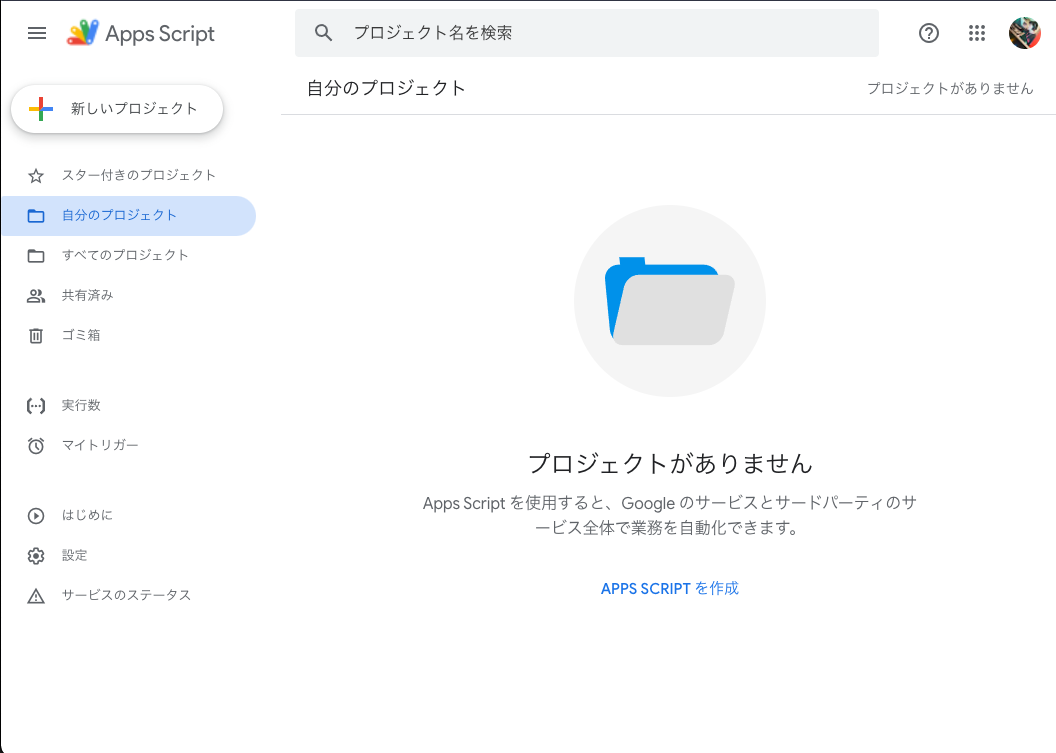
\includegraphics[keepaspectratio, scale=0.4]{images/gas_main.png}
 \caption{Google Apps Scriptメイン画面}
 \label{fig:gas_main}
\end{figure}

画面左上にある「新しいプロジェクト」ボタンをクリックすると,図\ref{fig:gas_edit}に示すようなエディタ画面が表示されます。Google Apps Scriptはこの画面上でプログラミングを行います\footnote{ローカルでの開発を可能にする\href{https://github.com/google/clasp}{Clasp}というツールもありますが,本テキストでは扱いません。}。

\begin{figure}[H]
 \centering
 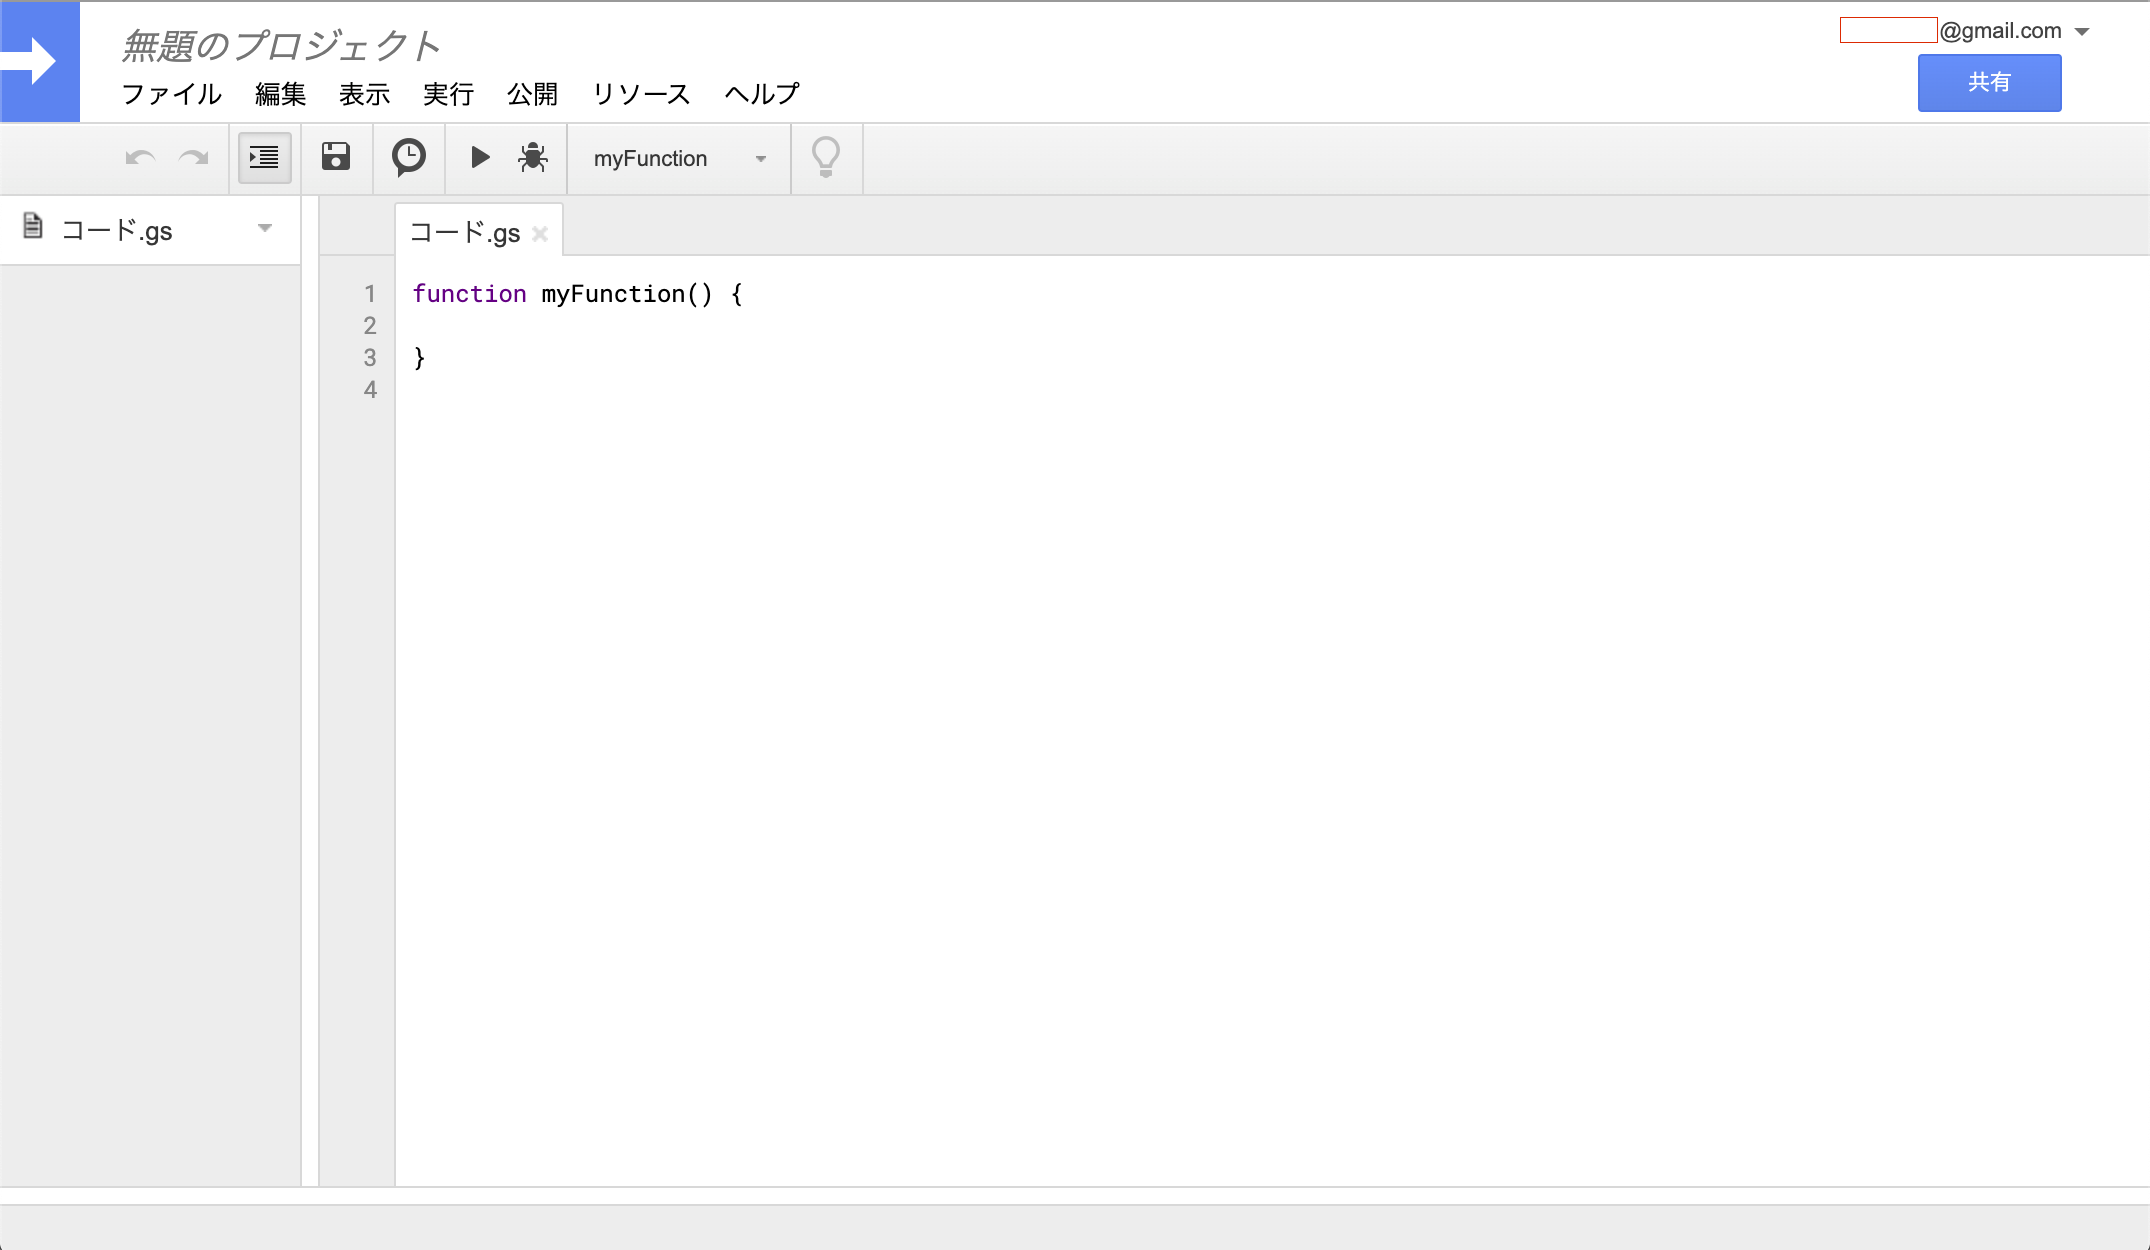
\includegraphics[keepaspectratio, scale=0.4]{images/gas_edit.png}
 \caption{Google Apps Script エディタ画面}
 \label{fig:gas_edit}
\end{figure}


加えて,なぜGoogle Apps Script単体でのHOW-TOではなく,Slackとの連携を主題に置いているか,といった点にも触れておきたいと思います。
GASはG Suiteを活用する上で非常に強力なツールですが,GAS以外の手段については意識したほうがよいでしょう。というのも,各Google Appsそれ自体にも多くの機能が備わっており,スクリプトを書くまでもなくGoogle Apps自体の機能で目的を実現できる場合もあるからです。

例として,「Google Spreadsheetsに入力された日本語の文章を英語に翻訳する」といったケースを考えてみます。先程説明したように,GASは各種Google Appsとシームレスに連携することができ,GASにはGoogle SpreadsheetsとGoogle TranslateへのAPIも含まれています。したがって,
\begin{enumerate}
\item Google Spreadsheets に入力されている日本語の文章を取得する
\item 取得された文章をGoogle Translateに流し込む
\item Google Translateによって翻訳された文章をGoogle Spreadsheetsに書き込む
\end{enumerate}
といった操作はGASを用いて以下のようなスクリプトを書くことで実現できます。

 \begin{lstlisting}[basicstyle=\ttfamily\footnotesize,frame=single,caption=Translate Script]
function translateSample() {

  var spreadsheet = SpreadsheetApp.openById('your/spreadsheet/id');
  var sheet = spreadsheet.getSheetByName('your/sheet/name');
  var ja_contents = sheet.getRange(2,1,sheet.getLastRow()-1).getValues();
  var translated_text = ""
  
  for (var i = 0; i < ja_contents.length; i++) {
    translated_text = LanguageApp.translate(ja_contents[i], 'ja', 'en');
    sheet.getRange(i+2, 2).setValue(translated_text);
  }
}
 \end{lstlisting}


さて,このようなケースでGASを用いるのは本当にベストな選択でしょうか?実は,Google Spreadsheetsには\href{https://support.google.com/docs/answer/3093331?hl=ja}{GOOGLETRANSLATEという関数が用意されています}。したがって,そもそもスクリプトを書く必要すらなく,Google Spreadsheetsの持つ機能だけで行いたかったことは実現できます\footnote{``翻訳の質''という観点で考えると,GASを用いた方法のほうが良い場合もあります。実際には実装コストと併せて考える必要があると思います。see: \href{https://qiita.com/kazinoue/items/82779a11af8a2dea0d21}{https://qiita.com/kazinoue/items/82779a11af8a2dea0d21}}。


上記の例ではGoogle SpreadsheetsとGoogle Translateの連携がGoogle Spreadsheetsだけで可能であることを説明しました。しかし,一般的には複数のGoogle Appsを組み合わせた処理はそれほど機能として用意されていません。なので,\textbf{複数のGoogle Appsを連携させる}用途,\textbf{Google Appsと外部サービスのAPIを連携させる}用途などではGASが効果を発揮する可能性が高いです。そのため,本テキストでも\textbf{Slackとの連携}を主軸に置いています。

\clearpage
\subsection{Incoming Webhooks とは}

\href{https://api.slack.com/messaging/webhooks}{Incoming Webhooks}はアプリケーションやプログラムからSlackにメッセージを投稿する方法(API)のひとつです。Webhook URLと呼ばれるURLに,投稿したい内容を持ったHTTPリクエストを送ると,Slack にメッセージが投稿されます。

\begin{itembox}[l]{APIとは}

API;Application Programming Interface とは,以下のように\href{http://e-words.jp/w/API.html}{説明されます}。

\begin{quote}
\textbf{API}とは、あるコンピュータプログラム(ソフトウェア)の機能や管理するデータなどを、外部の他のプログラムから呼び出して利用するための手順やデータ形式などを定めた規約のこと。
\end{quote}

上記の記述は抽象的なので,今回のテキストの内容に即して言葉を置き換えてみると,``\textit{Incoming Webhooks}とは,\textit{Slack}の機能や管理するデータなどを,\textit{GAS}をはじめとしたプログラムから呼び出して利用するための手順や規約''と考えることができます。


一方で,GAS自体もAPIと呼ぶことができます。この場合,「あるコンピュータプログラム」はGoogle Apps,「外部の他のプログラム」をGASと置き換えます。先程のスクリプトの例で登場した\textbf{SpreadsheetApp}や\textbf{LanguageApp}はそれぞれ,Google Spreadsheets,Google Translateを操作するためのオブジェクトですので,これらはAPIとなります。

特に,エンドポイントURLへのHTTPリクエストによって扱うAPIのことを,\textbf{Web API}と呼びます。したがって,Incoming WebhooksはWeb APIに該当します。

\end{itembox}

さて,Incoming Webhooksでは``投稿したい内容''をHTTPリクエストとして渡すとSlackにメッセージを投稿できるのでした。この``投稿したい内容''として必要な情報には何があるでしょうか?少なくとも,\textbf{投稿する内容(本文)}と\textbf{投稿する先(チャンネルやDM先)}は必要そうです。実は,Incoming Webhooksでは,図\ref{fig:webhook_sample}のように,通常私たちがSlackに投稿する形式以上の表現が可能です。そのため,Incoming Webhooksを使ってメッセージを投稿する際に指定できる情報は\textbf{本文}と\textbf{チャンネル}だけでなく,もっとたくさんありそうです。

\begin{figure}[h]
 \centering
 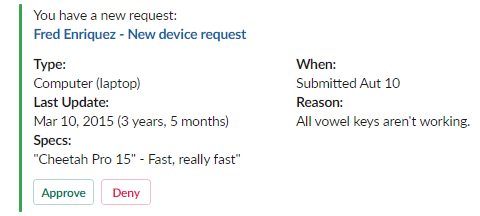
\includegraphics[keepaspectratio, scale=0.8]{images/webhook_sample.png}
 \caption{Incoming Webhooksによる投稿例}
 \label{fig:webhook_sample}
\end{figure}

現在,Slackには以下の2つの形式のIncoming Webhooksがあります。
\begin{enumerate}
\item Custom Integration\\
\textbf{カスタム インテグレーション}として設定するIncoming Webhooks。こちらでしか使えない機能もあるが,現在では非推奨の形式。
\item App\\
\textbf{Slack App}として設定するIncoming Webhooks。現在はこちらが推奨されている。
\end{enumerate}

それぞれの形式のIncoming Webhooksについて詳しく説明します。

\subsubsection{Custom Integration(Legacy)}

Slackでは,よく使いそうな機能が組み込みのアプリケーションとして用意されており,必要に応じて用途に即した形で設定を追加できます。これを\textbf{カスタムインテグレーション}といいます。\textbf{よく使いそうな機能}には,Incoming WebhooksのほかにOutgoing WebhooksやSlash Commandsなどがあります。

設定済みのカスタムインテグレーションは,\\
\verb|https://{ワークスペース名}.slack.com/apps/manage/custom-integrations|\\
から確認できます。

\begin{figure}[h]
 \centering
 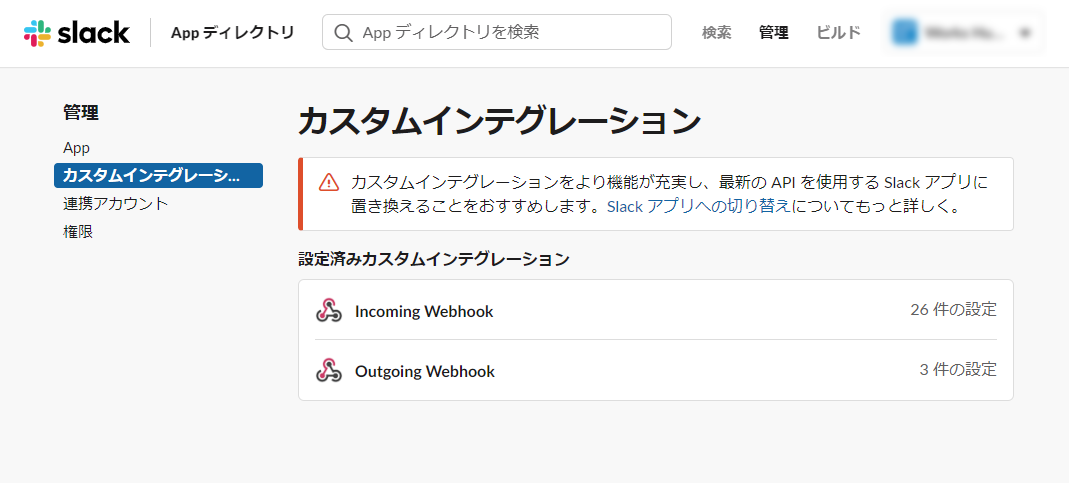
\includegraphics[keepaspectratio, scale=0.6]{images/custom_integration1.png}
 \caption{カスタムインテグレーション画面1}
 \label{fig:custom_integration1}
\end{figure}

カスタムインテグレーションは,後述する理由により現在では\textbf{非推奨}の形式ですので,上記の画面上にも\textbf{Slackアプリに置き換えることをおすすめします。}と記載されています。


Incoming Webhooksの設定を追加する場合は,この画面上でIncoming Webhooksと書かれている部分を選択します。

\begin{figure}[h]
 \centering
 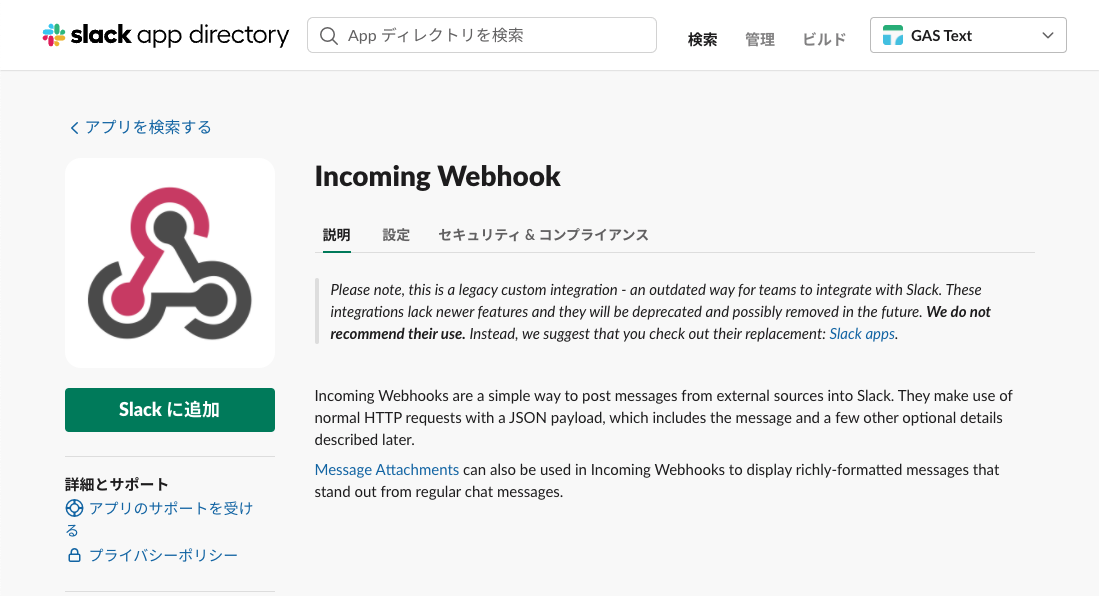
\includegraphics[keepaspectratio, scale=0.6]{images/custom_integration2.png}
 \caption{カスタムインテグレーション画面2}
 \label{fig:custom_integration2}
\end{figure}

画面上に\textbf{設定をリクエストする}といったボタンが表示されています。これをクリックすると,Slackワークスペースの管理者に設定の追加をリクエストすることができます。ちなみに,このボタンが\textbf{設定を追加}になっている場合は,管理者の承認を必要とせず,自由に設定を追加できます。


カスタムインテグレーションのIncoming Webhooksに\textbf{デフォルトの}チャンネルやユーザー名・アイコンなどを決めた設定を追加すると,独自のURLが発行されます。このURLがWebhook URLです。このURLに対して,投稿したい内容を持ったHTTPリクエストを送ると,事前に設定したデフォルトのチャンネルに対して,デフォルトのユーザー名・アイコンで投稿が行われます。


なお,このデフォルトのチャンネルやユーザー名,アイコンはいつでも変更できます。

\clearpage
カスタムインテグレーションのIncoming Webhooksでのみ可能な使い方として,\textbf{投稿先のチャンネル,投稿のユーザー名,アイコンを自由に変えられる}ことが挙げられます。

先程説明したように,投稿する内容のみを使ってWebhook URLに対してPOSTを行うと,デフォルトのチャンネルに対して投稿が行われます。
例として,以下のCurlコマンドの実行例を見てみます。

\begin{lstlisting}[basicstyle=\ttfamily\footnotesize,language=command.com,frame=single,caption=Curl sample]
> curl -X POST --data-urlencode "payload={\"text\": \"TEST\" }" https://hooks.slack.com/services/your/webhook/url
ok
\end{lstlisting}

\begin{figure}[h]
 \centering
 
\includegraphics[keepaspectratio, scale=0.8]{images/webhook_sample2.png}
 \caption{Incoming Webhooks実行例}
 \label{fig:webhook_sample2}
\end{figure}

図\ref{fig:webhook_sample2}では,事前に設定したデフォルトのユーザー名(\verb|TSD CI webhook|)で投稿されています。アイコンは設定していないため,カスタムインテグレーションのアイコンが表示されています。

ここで,Webhook URLに送信する情報(上記Curlコマンドのpayload要素)をいくつか追加してみましょう。

\begin{lstlisting}[basicstyle=\ttfamily\footnotesize,language=command.com,frame=single,caption=Curl sample2]
> curl -X POST --data-urlencode "payload={\"text\": \"TEST\", \"channel\": \"@shimada_ken\", \"username\": \"This is custom integration\", \"icon_emoji\": \":tada:\" }" https://hooks.slack.com/services/your/webhook/url
ok
\end{lstlisting}

payload要素が長くなりすこし見づらくなってしまいました。payloadの部分だけ見やすく整形すると以下のようになります。

\begin{lstlisting}[basicstyle=\ttfamily\footnotesize,frame=single,caption=Formed payload,label=formedpayload]
payload = {
  "text": "TEST",
  "channel": "@shimada_ken",
  "username": "This is custom integration",
  "icon_emoji": ":tada:"
}
\end{lstlisting}

ここでは,\verb|text|の他に,\verb|channel|,\verb|username|,\verb|icon_emoji|を設定しています。それぞれ,送信先のチャンネル,表示名,アイコンとなる絵文字に対応します。
上記Curlコマンドを実行すると,以下のような内容が私にダイレクトメッセージで送信されます。ユーザー名が\verb|TSD CI webhook|から\verb|This is custom integration|に,アイコンがクラッカーの絵文字になっていることがわかります。カスタムインテグレーションのIncoming Webhooksでは,アイコンをSlackの絵文字で代替することができます。もちろん,画像を指定することも可能です。

\begin{figure}[h]
 \centering
 
\includegraphics[keepaspectratio, scale=0.8]{images/webhook_sample3.png}
 \caption{Incoming Webhooks実行例2}
 \label{fig:webhook_sample3}
\end{figure}

このように,送信先やユーザー名,アイコンを自由に変えられるのが,カスタムインテグレーションのIncoming Webhooksの特徴です。そのため,\textbf{1つのWebhook URLで様々なプログラム・アプリケーションに対応できます}。

\subsubsection{App(Recommended)}

一方で,1つのWebhook URLには1つの役割しか与えないほうがよい,という考えがあります。なぜなら,あるカスタムインテグレーションによって作成されたWebhook URLがあったとき,これがどのプログラム・アプリケーションに使われているのか把握できないといった問題が発生するからです。カスタムインテグレーションのWebhook URLは,任意のチャンネルに対して,任意の見た目(ユーザー名やアイコン)で投稿ができてしまうので,極端な話をするとこれは1つのワークスペースに1つあればよいということになってしまいます。つまり,カスタムインテグレーションによるIncoming Webhooksでは,Webhook URLと実際にURLが使用されるアプリケーション間の関係といった情報が欠落してしまっているのです。

そこで,Slack Appの一部としてのIncoming Webhooksが登場します。これは,Slack Appとしてワークスペースに設定するので,そのAppの役割に即して使われる想定で存在します。当然,Appの役割は決まっており,ユーザー名やアイコン,投稿するチャンネルが変わることはないはずです。ですので,このIncoming Webhooksではこれらを変えることができません。1つのWebhook URLには必ず1つのチャンネルが結びついており,例外はありません。もし1つのAppが複数のチャンネルに投稿しなければならない場合は,AppからWebhook URLを\textbf{投稿先の数だけ}発行します。

AppとしてIncoming Webhooksを利用する手順は以下の通りとなります。

\begin{enumerate}
\item Slack Appの作成
\item Incoming Webhooksの有効化
\item Incoming Webhooksの作成
\end{enumerate}

まず,Slack Appを作成します。これは\href{https://api.slack.com/apps?new_app=1}{https://api.slack.com/apps?new\_app=1}から作成できます。このURLにアクセスすると,以下の図\ref{fig:create_new_app}のような画面が表示されます。

\begin{figure}[H]
 \centering
 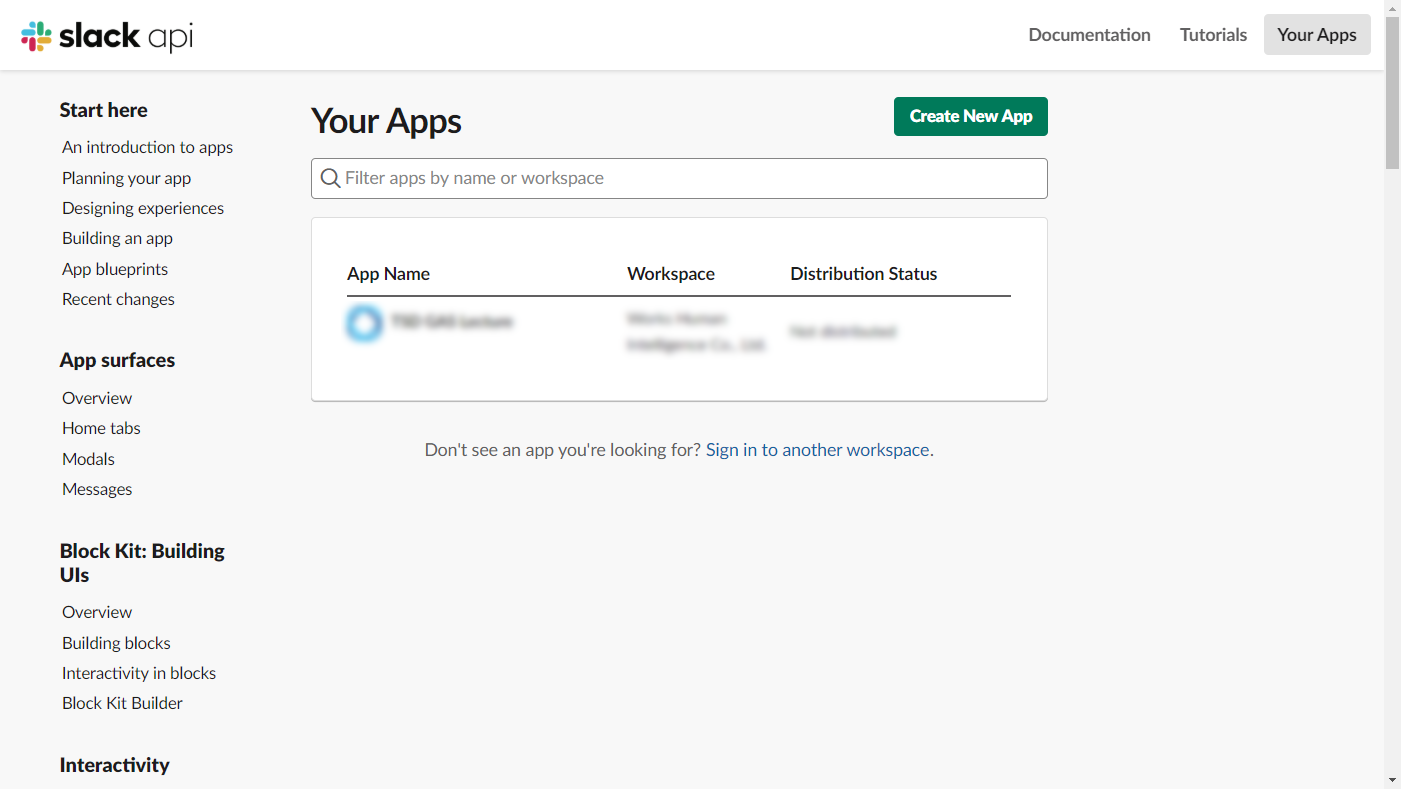
\includegraphics[keepaspectratio, scale=0.45]{images/create_new_app.png}
 \caption{App作成画面}
 \label{fig:create_new_app}
\end{figure}

この画面右上の``Create New App''というボタンをクリックすると,図\ref{fig:create_new_app2}のダイアログが表示されます。ここに,作成するApp名と,Appを設定するワークスペースを入力し,``Create App''ボタンをクリックします。ワークスペースのポリシーにより,Appの設定に管理者の承認が必要な場合は,このタイミングで管理者にリクエストが送られます。特に承認が不要な場合は,そのままAppが作成されます。

\begin{figure}[H]
 \centering
 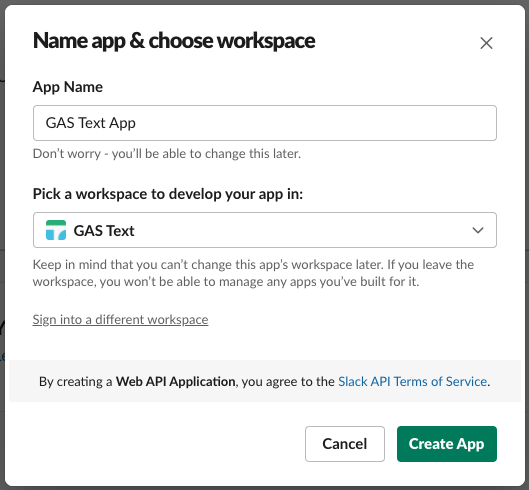
\includegraphics[keepaspectratio, scale=0.55]{images/create_new_app2.png}
 \caption{App作成画面2}
 \label{fig:create_new_app2}
\end{figure}

Appが作成されると,Appごとに図\ref{fig:create_new_app3}のような画面を見ることができます。まず,この画面下部の``\textbf{Display Information}''から,このAppがSlackに投稿する際のユーザー名とアイコンを設定します。Incoming Webhooksで投稿する際もここで設定したユーザー名とアイコンが使用されます。

\verb|App name|の部分に設定したいユーザー名を入力して,ユーザー名を設定します。\\
次に,アイコンの部分をクリックし,画像をアップロードしてアイコンを設定します。なお,ここで設定する画像は 512px x 512px から 2000px x 2000px に収まる正方形の画像である必要があります。ちなみに,カスタムインテグレーションの場合はEmojiをアイコンに設定できましたが,Appでは画像のみとなります。


設定後,画面下部の\textbf{Save Changes}をクリックして設定を反映します。

\begin{figure}[H]
 \centering
 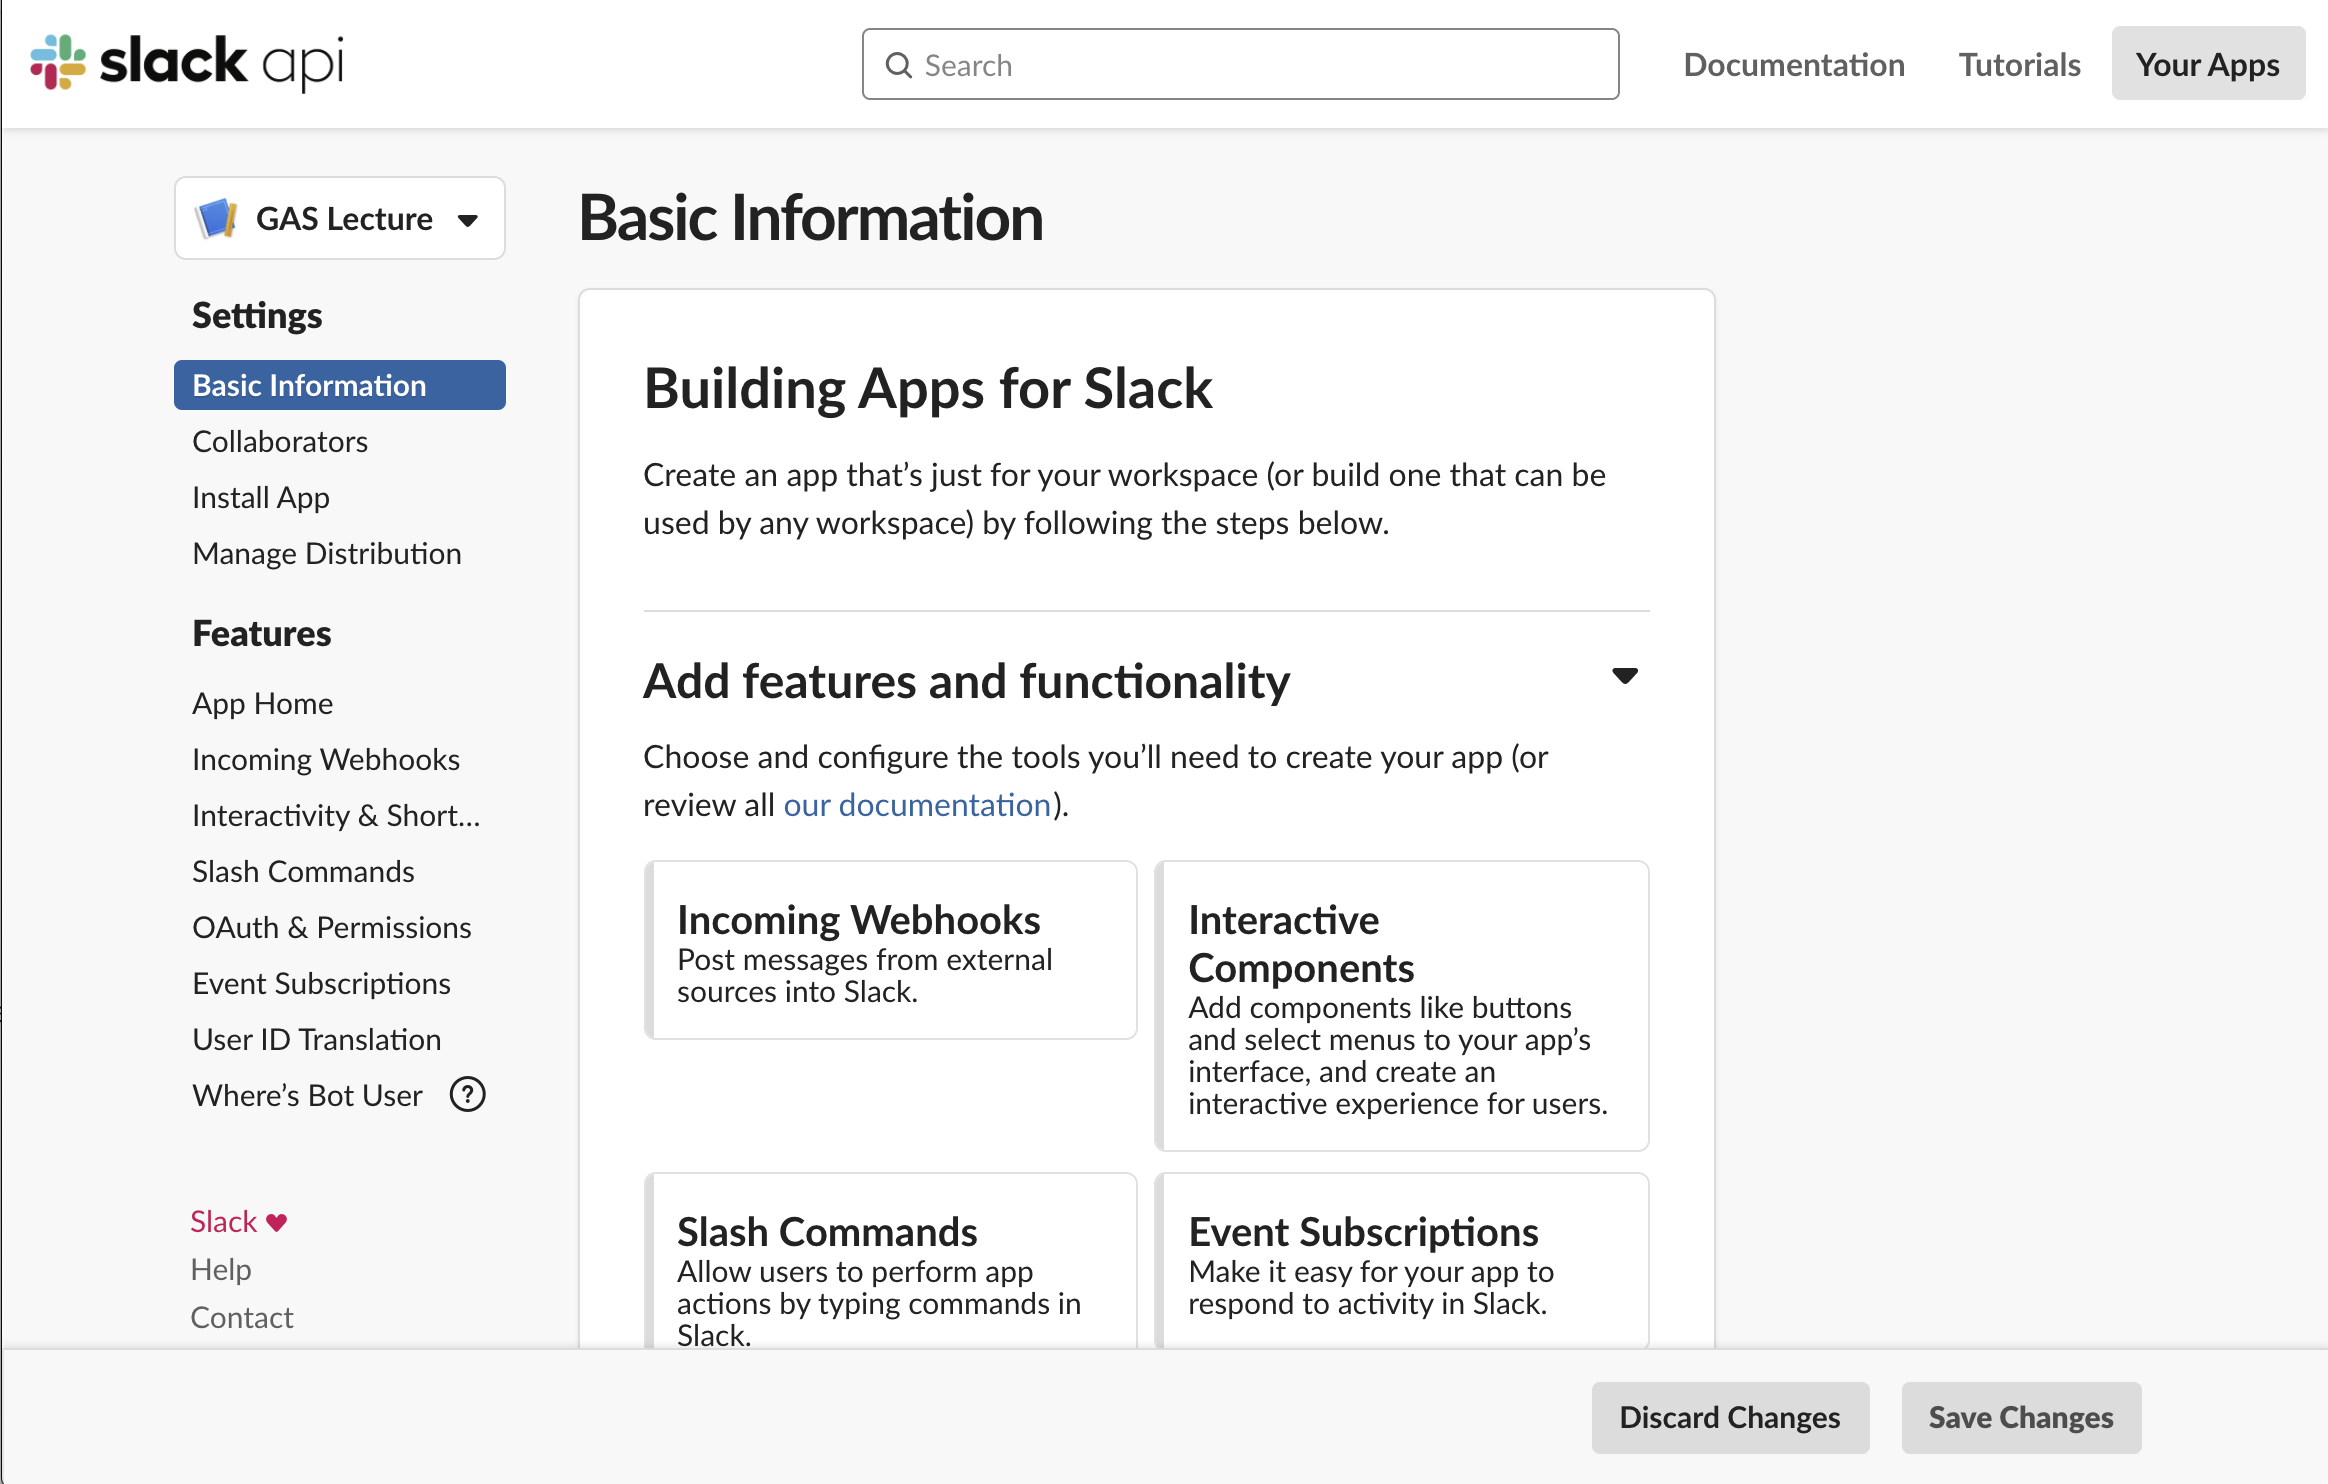
\includegraphics[keepaspectratio, scale=0.4]{images/create_new_app3.png}
 \caption{App画面}
 \label{fig:create_new_app3}
\end{figure}

\begin{figure}[H]
 \centering
 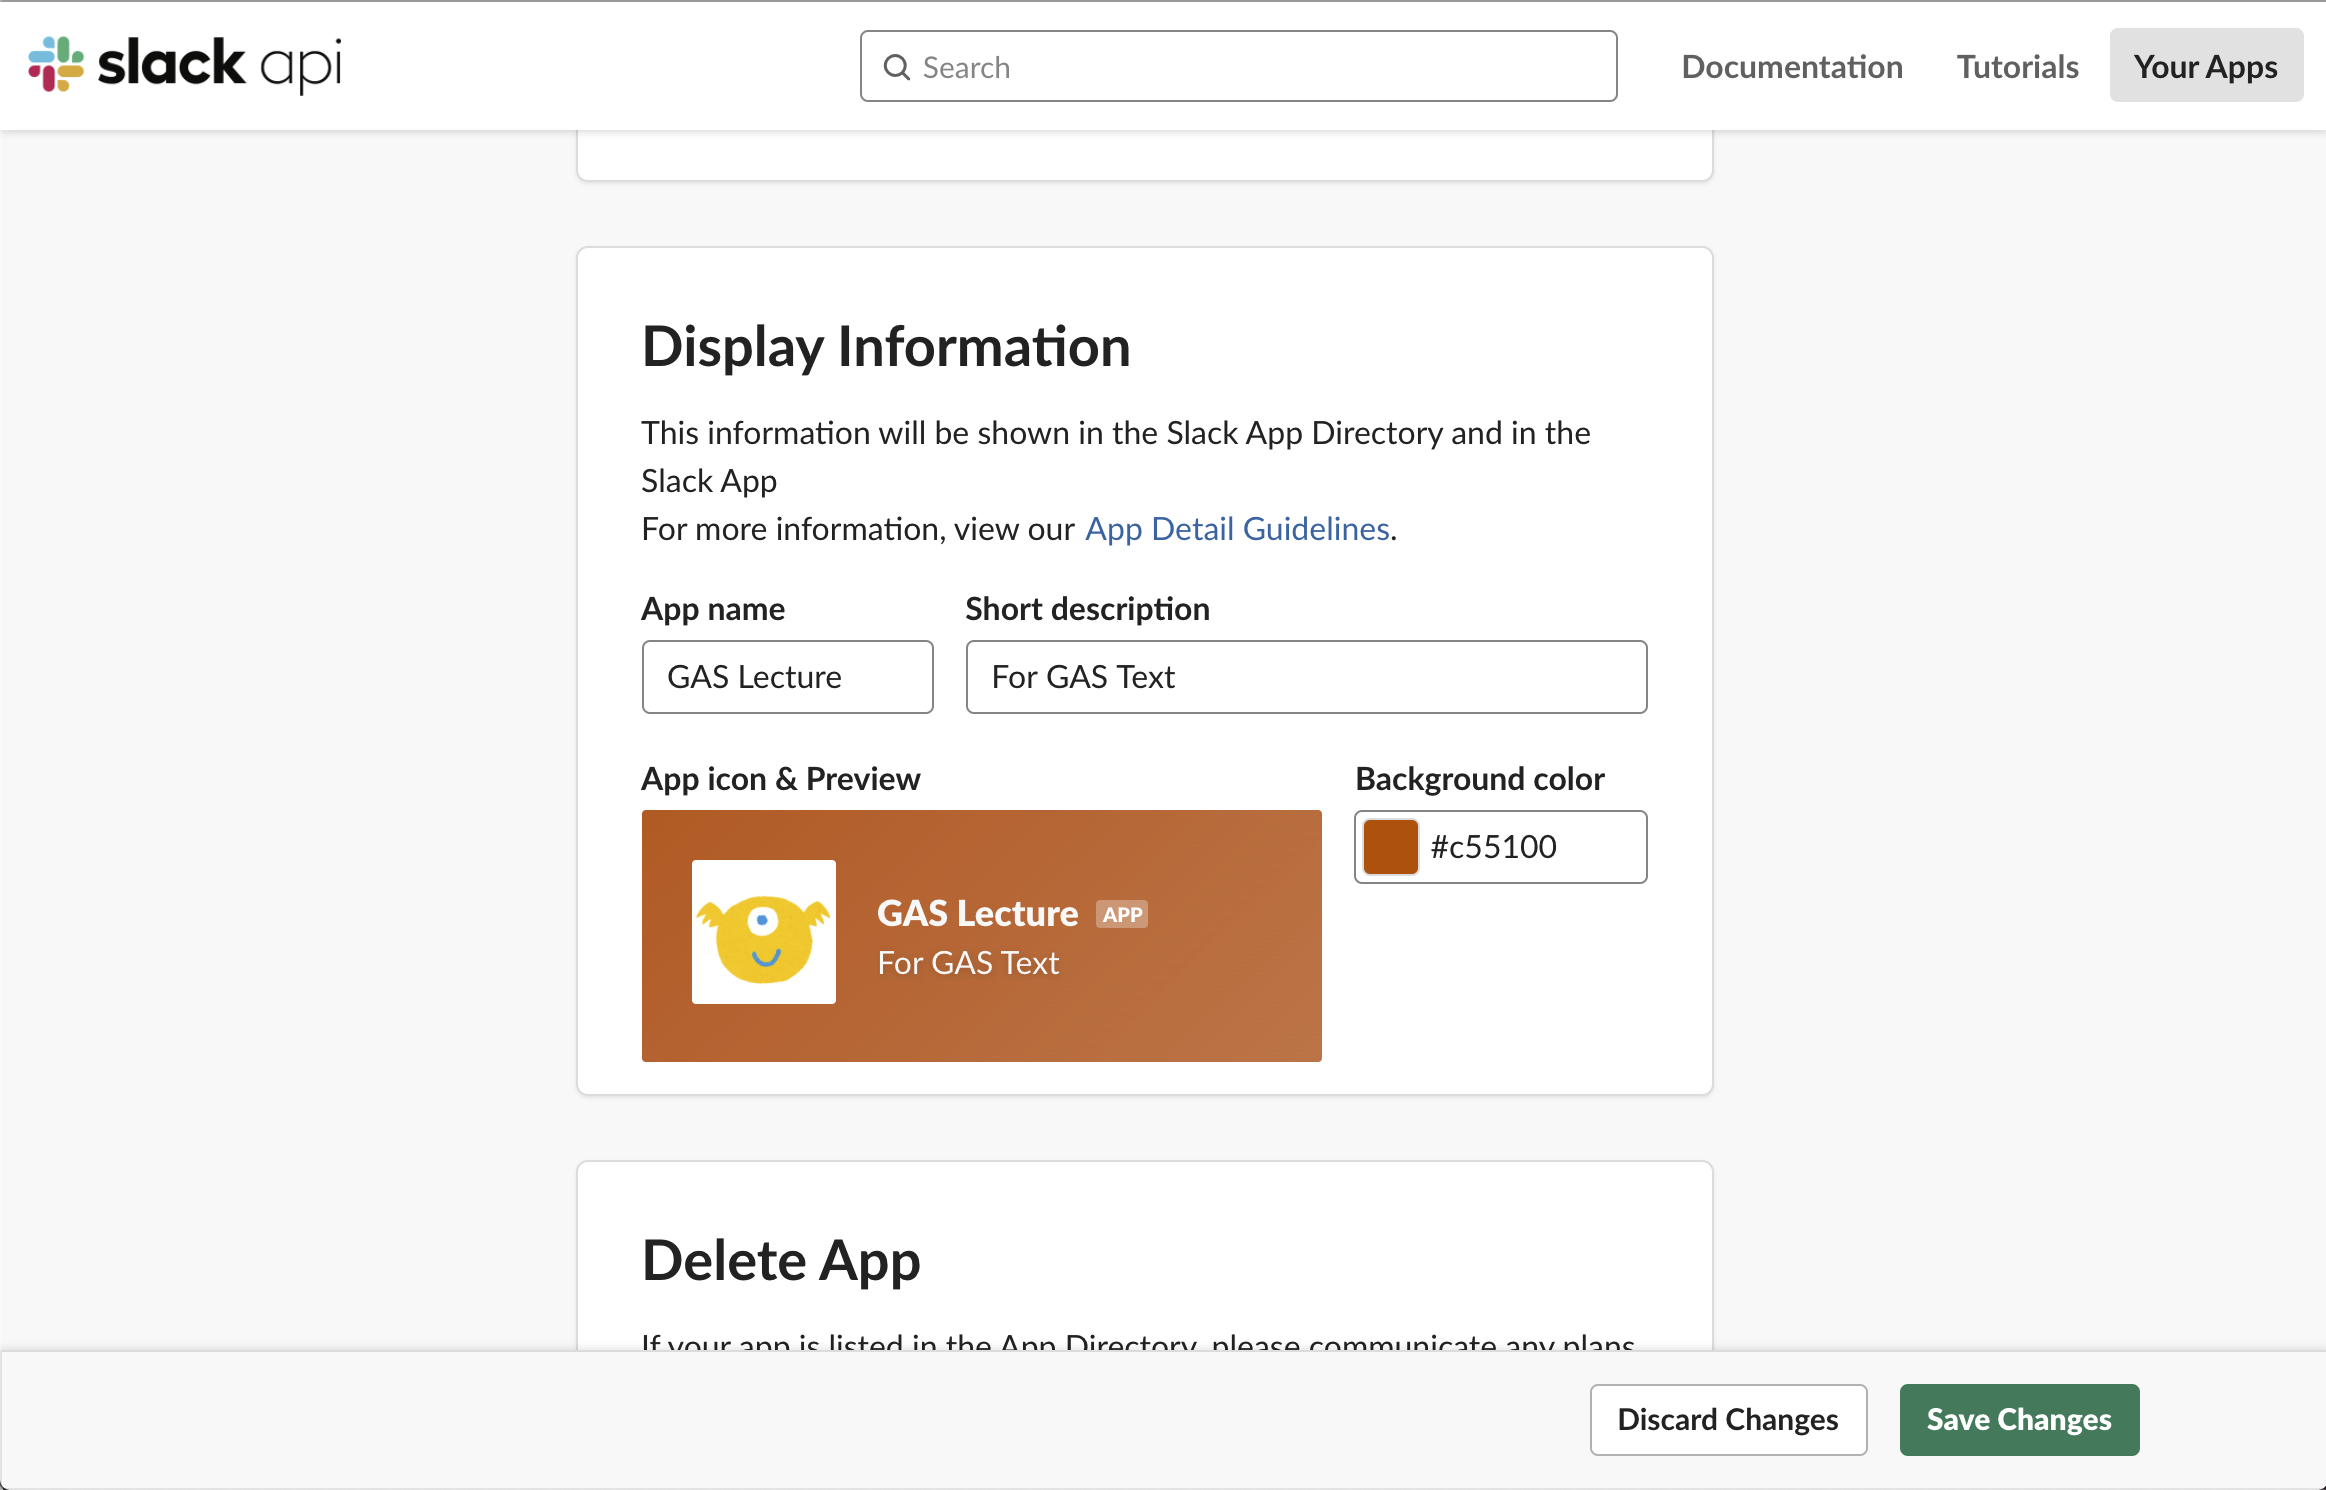
\includegraphics[keepaspectratio, scale=0.5]{images/create_new_app5.png}
 \caption{App画面,Display Information部分}
 \label{fig:create_new_app5}
\end{figure}

引き続き,Incoming Webhooksの設定を行っていきましょう。この画面左カラムに,``Incoming Webhooks''というメニューがありますので,こちらを選択します。
``Incoming Webhooks''を選択すると,図\ref{fig:create_new_app4}のような画面が開きます。はじめは,画面右上のスイッチが\textbf{Off}になってますので,ここをクリックし,Incoming Webhooksを有効にします。Incoming Webhooksが有効になると,図\ref{fig:create_new_app4}の画面になります。画面下部の``Add New Webhook to Workspace''(Webhookの追加に管理者の承認が必要な場合は``Request to Add New Webhook'')をクリックして,Webhook URLを発行します。

\begin{figure}[H]
 \centering
 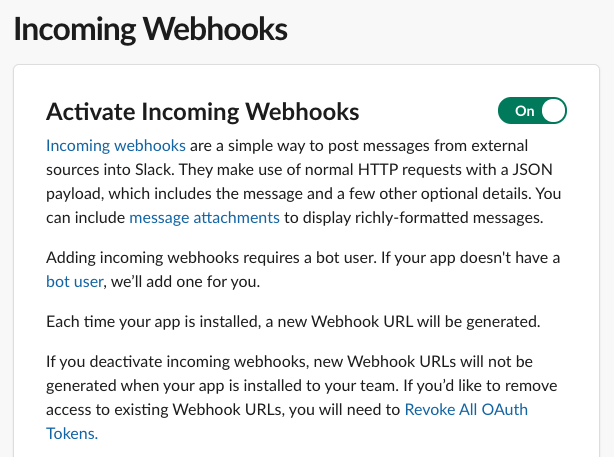
\includegraphics[keepaspectratio, scale=0.6]{images/create_new_app4.png}
 \caption{Incoming Webhooks画面(App)}
 \label{fig:create_new_app4}
\end{figure}

``Add New Webhook to Workspace''をクリックすると,投稿するチャンネル名を指定する画面に遷移します。投稿するチャンネル名を選択し,``Install''(管理者の承認が必要な場合は``許可する'')ボタンをクリックします。

\begin{figure}[H]
 \centering
 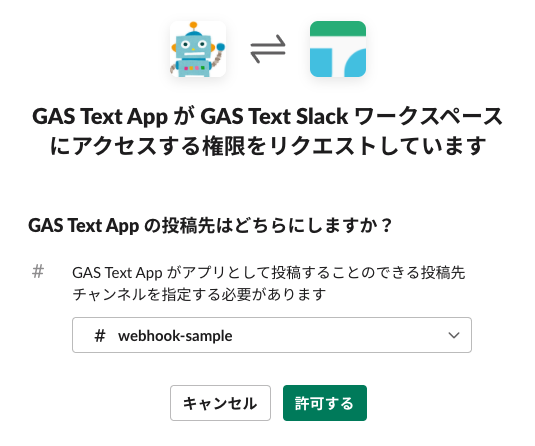
\includegraphics[keepaspectratio, scale=0.6]{images/create_incoming_webhooks.png}
 \caption{Incoming Webhooks画面(App)}
 \label{fig:create_new_app4}
\end{figure}

すると,図\ref{fig:create_new_app4}の画面に,設定したチャンネルへ投稿するためのWebhook URLが表示されます。GASからSlackへ投稿するために,このURLを控えておきます。なお,このURLはApp画面でいつでも確認できます。

\clearpage
\section{単独で動作するGoogle Apps Script}

前章では,Google Apps Scriptを利用する画面へのアクセス方法と,Incoming WebhooksのWebhook URL発行方法について説明しました。ここからは,実際にGoogle Apps ScriptとIncoming Webhooksを使ってみましょう。といっても,この章ではGoogle Appsとの連携は行いません。まずは単体のGoogle Apps ScriptからIncoming Webhooksを使ってSlackにメッセージを投稿してみましょう。

なお,本章以降で使用するWebhook URLはカスタムインテグレーションから発行したものではなく,Appから発行したものを使用します。

\paragraph{本章で扱うトピック}
\begin{itemize}
\item Google Apps Scriptの実行方法
\item ロガー
\item オブジェクトとJSON
\item UrlFetchApp
\end{itemize}

\subsection{Example: GASからIncoming Webhooksを使ってSlackに投稿してみよう}

本節では,Google Apps ScriptからIncoming WebhooksのWebhook URLに対してPOSTリクエストを行い,Slackにメッセージを送信します。\ref{subsec:About GAS}にて紹介した経路で,Google Apps Scriptのプロジェクトを作成します。

プロジェクトを作成すると,以下のようなスクリプトコードが既に入力された状態でエディタ画面が開きます。

\begin{lstlisting}[basicstyle=\ttfamily\footnotesize,frame=single,caption=Default Script]
function myFunction() {

}
\end{lstlisting}

\verb|myFunction|という空の関数が定義されている状態です。関数名が\verb|myFunction|では何をする関数かわかりづらいので,この関数名を変えておきましょう。本テキストでは,\verb|slackSender|という名前をつけますが,好きな名前をつけてよいです。

\begin{lstlisting}[basicstyle=\ttfamily\footnotesize,frame=single,caption=Change function name]
function slackSender() {

}
\end{lstlisting}

\subsubsection{スクリプトの実行方法とロギング}

まずはGASの実行方法を紹介します。ですが,まだ\verb|slackSender|関数にはなにも処理を書いていないので,当然このまま実行するとなんの処理も実行されません。なので,実行できていることを確認するために,ログ出力を記述します。ログ出力は,\verb|Logger.log()|で行えます。いわゆるJavaScriptにおける\verb|console.log()|のようなものです。\verb|Logger.log()|は,文字列を渡せば文字列が表示されますし,変数を渡せばその中身が表示されます。

ひとまず実行できていることが確認できればよいので,以下のようにログ出力を記述します。中に入る文字列は当然なんでもよいです。

\begin{lstlisting}[basicstyle=\ttfamily\footnotesize,frame=single,caption=Logging]
function slackSender() {
  Logger.log("My first logging!!");
}
\end{lstlisting}


上記のようにスクリプトが書けたら,実行してみましょう。実行は,エディタ画面上部にあるツールバーの,再生ボタン(▶ボタン)をクリックします。複数の\verb|function|が定義されている場合は,実行する\verb|function|を右側のドロップダウンから選択できます。

\begin{figure}[H]
 \centering
 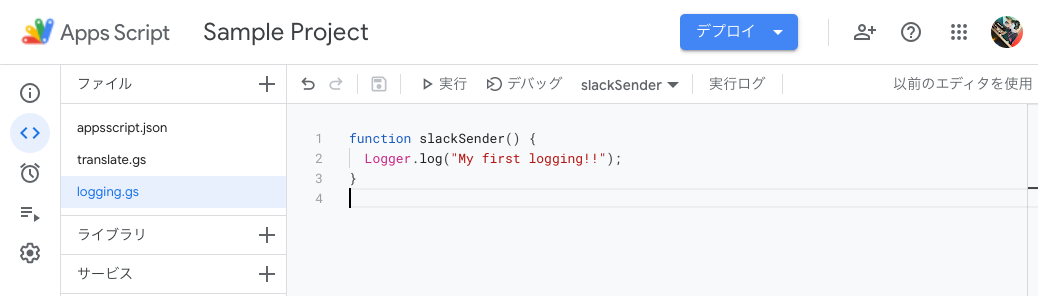
\includegraphics[keepaspectratio, scale=0.7]{images/standalone_gas1.png}
 \caption{GASツールバー}
 \label{fig:standalone_gas1}
\end{figure}

初めての実行時,\textbf{Authorization required}といったタイトルのダイアログが表示されます。これは,「このスクリプトを実行していいですか?」という確認と,それをユーザーのG Suiteアカウントから承認するダイアログです。画面の指示に従って承認してください。詳しくは,\href{https://tonari-it.com/gas-script-approval/}{こちら}のウェブサイトが詳しいので,必要に応じて参照してください。

実行が完了したら,ログを確認してみましょう。ログは,ツールバーの\textbf{表示}から\textbf{ログ}をクリックするか,\verb|Ctrl+Enter|で表示できます。正常に実行できていれば,以下の図\ref{fig:standalone_gas2}のようにログが出力されています。\verb|Logger.log()|を使ったログ出力はスクリプトのデバッグによく使用するので,覚えておきましょう。

\begin{figure}[H]
 \centering
 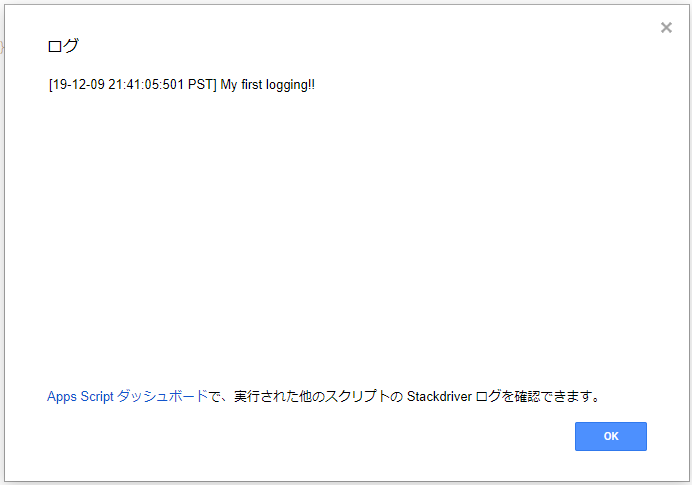
\includegraphics[keepaspectratio, scale=0.7]{images/standalone_gas2.png}
 \caption{ログ出力例}
 \label{fig:standalone_gas2}
\end{figure}

\subsubsection{UrlFetchAppとWeb APIへのHTTPリクエスト}


ここから本格的にGoogle Apps Script上でIncoming Webhooksを利用していきます。これまで,Incoming Webhooksを「Webhook URLに投稿したい内容を持ったHTTPリクエストを送ると,Slack にメッセージが投稿できる」と説明していました。ここからは「投稿したい内容を持ったHTTPリクエスト」を送る具体的な方法について説明していきます。

Google Apps Scriptでは,\href{https://developers.google.com/apps-script/reference/url-fetch/url-fetch-app}{UrlFetchApp}というクラスでHTTPリクエストを行います。このクラスでは,ウェブを介したHTTPリクエストと,そのレスポンスの取得が行えます。HTTPリクエストを送るには,\href{https://developers.google.com/apps-script/reference/url-fetch/url-fetch-app#fetchurl,-params}{UrlFetchApp.fetch(url, params)}を使用します。今回,リクエストを送る先のURLはWebhook URLに対応しますので,\verb|url|引数にはこれを入力します。\verb|param|引数については後述します。


さて,リクエストを受け取る側(Slackのサーバー)もプログラムで動いていますので,闇雲にHTTPリクエストを送ってもサーバー側は解釈できません。リクエストの形式には決まり(プロトコル)が定められています。2019年現在,Webサービスの提供するWeb APIの多くはJSONを受け取り,JSONを返すように作られています。Incoming Webhooksでも,送信したい内容のJSONを送ることで,Slackのサーバー側が正しく解釈でき,メッセージを投稿できます。


Incoming Webhooksに渡すJSONのうち,最も単純なものは以下に示すような「投稿したいメッセージ」のみを持ったJSONです。これをWebhook URLに対して送ると,デフォルトのSlackチャンネルにメッセージが送信されます。
\begin{lstlisting}[basicstyle=\ttfamily\footnotesize,frame=single,caption=Minimum JSON payload for Incomming Webhooks,label=jsonpayload]
{
  "text": "This is the message"
}
\end{lstlisting}

Slackのサーバー側へ命令を送る際の決まりは,JSONで送ることでしたが,その「送る」を担う\textbf{HTTPリクエスト}にも決まりが存在します。この「決まり」に即してパラメータを設定する部分が,冒頭で紹介した\verb|UrlFetchApp.fetch(url, params)|の\verb|params|引数に対応します。ここで必要になるのは,「JSON形式でこの(上記のJSON)データを送りますよ」ということの宣言です。この宣言は,以下のように分割することができ,またそれぞれが\verb|params|引数のパラメータに対応します。

\begin{itemize}
\item JSON形式で\\
→\verb|headers|パラメータに対応
\item このデータを\\
→\verb|payload|パラメータに対応
\item 送りますよ\\
→\verb|method|パラメータに対応
\end{itemize}


まず,「送ります」は\verb|POST|というリクエストメソッドに対応します。ここでは\verb|method|に\verb|POST|を指定すればいいんだなー程度で大丈夫です。リクエストメソッドについて気になる方は各自調べていただければと思います。HTTPリクエストメソッドには他に\verb|GET, PUT, DELETE|などがあり,Web APIではこれらのメソッドによってサービスに対する操作を区別することが多いです。


「JSON形式」を宣言するには,リクエストヘッダに\verb|Content-type|を指定します。JSON形式に対応する\verb|Content-type|は\verb|application/json|です。リクエストヘッダについて気になる方は(以下略)


したがって,以下のような形式になります。

\begin{lstlisting}[basicstyle=\ttfamily\footnotesize,frame=single,caption=params argument for UrlFetchApp]
{
  "method": "POST",
  "headers": {"Content-type": "application/json"}
}
\end{lstlisting}

さて,あとはソースコード\ref{jsonpayload}に示したJSONオブジェクト(実際にAPIに対して渡すデータ)を\verb|params|引数に含めれば,\verb|params|に渡すべきオブジェクトは完成します。これは,\verb|payload|パラメータに設定するのですが,\verb|payload|パラメータに設定できるのは文字列のみです。そこで,先のJSONオブジェクト全体を文字列に変換する必要があります。これは,JavaScript組み込みの\verb|JSON.stringify|という関数で変換できます。あるJSONオブジェクト\verb|obj|をJSON文字列に変換するには,この関数に\verb|obj|を渡してやればよいので,\verb|JSON.stringify(obj)|となります。したがって,スクリプト全体は以下のようになります。\verb|your/webhook/url|の部分は実際に取得したWebhook URLを入力します。

\begin{lstlisting}[basicstyle=\ttfamily\footnotesize,frame=single,caption=Incoming Webhooks Sample]
function slackSender() {
  
  var payload = {
    "text": "This is the message"
  }
  
  var options = {
    "method": "POST",
    "headers": {"Content-type": "application/json"},
    "payload": JSON.stringify(payload)
  };
        
  UrlFetchApp.fetch("your/webhook/url", options);
  
}
\end{lstlisting}

上記スクリプトを実行すると,以下のようにSlackに投稿されます。

\begin{figure}[H]
 \centering
 
\includegraphics[keepaspectratio, scale=1.0]{images/standalone_gas3.png}
 \caption{スクリプト実行例}
 \label{fig:standalone_gas3}
\end{figure}


\subsection{いろいろなPayloadの作成と実行例}


前節では,\verb|text|に単純な文字列を指定して,シンプルなメッセージ投稿を行いました。しかし,Incoming Webhooksでは,通常私たちがSlackの画面から投稿するよりもリッチな投稿ができます。この節ではその例について紹介します。

\subsubsection{mrkdwn記法}


通常私たちがSlackのメッセージを投稿するときも使用できるように,SlackにはMarkdownに似た記法でテキストの装飾ができます。この記法を\textbf{mrkdwn}と呼びます。


たとえば,図\ref{fig:mrkdwn_sample}に示すように,\verb|*bold*|と文字列を\verb|*|で囲むと,囲まれた文字列が太字になったり,\verb|`code`|と文字列を\verb|`|(バッククオート)で囲むと,囲まれた文字列がコードテキストになったりするものです。

\begin{figure}[H]
 \centering
 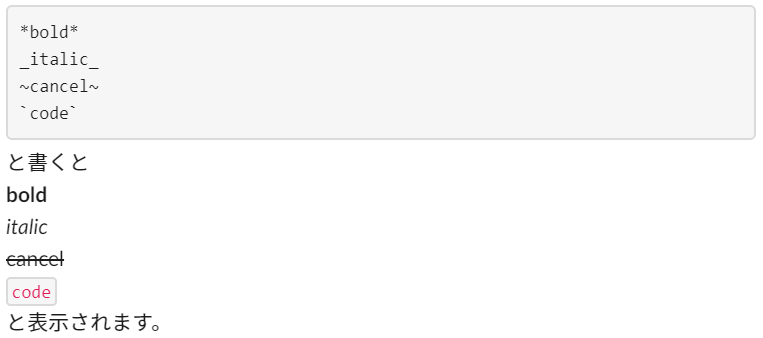
\includegraphics[keepaspectratio, scale=0.8]{images/mrkdwn_sample.png}
 \caption{mrkdwn記法の例}
 \label{fig:mrkdwn_sample}
\end{figure}

これはIncoming Webhooksでメッセージを投稿する場合も有効で,実際以下のソースコード\ref{mrkdwnpayload}のようなpayloadでメッセージを投稿すると,図\ref{fig:mrkdwn_payload1}のように表示されます。

\begin{lstlisting}[basicstyle=\ttfamily\footnotesize,frame=single,caption=mrkdwn payload sample,label=mrkdwnpayload]
{
  "text": "*This* is a _sample_ of `mrkdwn` ~notation~"
}
\end{lstlisting}

\begin{figure}[H]
 \centering
 
\includegraphics[keepaspectratio, scale=0.8]{images/mrkdwn_payload1.png}
 \caption{mrkdwn記法を使ったメッセージ投稿例}
 \label{fig:mrkdwn_payload1}
\end{figure}


\subsubsection{メンション}

前項では,Slackの画面から通常通りメッセージを投稿するように,Incoming Webhooksでもメッセージの装飾ができることを紹介しました。一方,\verb|@here|,\verb|@channel|,\verb|@everyone|を含む,メンションには少し注意が必要です。


たとえば,私(\verb|@hitsumabushi845|)にメンションを飛ばそうと思い,以下のようなpayloadを作成したとします。

\begin{lstlisting}[basicstyle=\ttfamily\footnotesize,frame=single,caption=mention payload sample1,label=mrkdwnpayload]
{
  "text": "@hitsumabushi845 mention...?"
}
\end{lstlisting}

このpayloadを使ってIncoming Webhooksでメッセージを投稿すると,以下のように正しくメンションにならず,\verb|@hitsumabbushi845|は単なる文字列として表示されてしまいます。

\begin{figure}[H]
 \centering
 
\includegraphics[keepaspectratio, scale=0.8]{images/mention1.png}
 \caption{Incoming Webhooksを使ったメンション(失敗例)}
 \label{fig:mention1}
\end{figure}

これを正しくメンションとして表示するためには,以下のように\verb|@username|を\verb|<>|で囲む必要があります。なお,\verb|@username|を\verb|<>|で囲むメンションは〜〜

\begin{lstlisting}[basicstyle=\ttfamily\footnotesize,frame=single,caption=mention payload sample2,label=mrkdwnpayload]
{
  "text": "<@hitsumabushi845> mention!"
}
\end{lstlisting}

こうすることで,正しくメンションとしてメッセージが投稿されます。

\begin{figure}[H]
 \centering
 
\includegraphics[keepaspectratio, scale=0.8]{images/mention2.png}
 \caption{Incoming Webhooksを使ったメンション(成功例)}
 \label{fig:mention2}
\end{figure}

同様に,\verb|@here|,\verb|@channel|,\verb|@everyone|も\verb|<@here>|,\verb|<@channel>|,\verb|<@everyone>|となる・・・かと思いきや,これらは\verb|<!here>|,\verb|<!channel>|,\verb|<!everyone>|です。

\begin{table}[H]
  \caption{Incoming Webhooksでのメンション対応表}
  \centering
  \begin{tabular}{l|ll}
対象 & 通常 & Incoming Webhooks \\ \hline
個別のユーザー & \verb|@username| & \verb|<@username>| \\
チャンネルに参加しているオンライン状態のユーザー全員 & \verb|@here| & \verb|<!here>| \\
チャンネルに参加しているユーザー全員 & \verb|@channel| & \verb|<!channel>| \\
ワークスペースに参加しているユーザー全員\footnotemark & \verb|@everyone| & \verb|<!everyone>| \\
  \end{tabular}
\end{table}
\footnotetext{\verb|@everyone|はワークスペース全体が参加するチャンネル(\verb|#general, #random|など)でのみ使うことができます。}


なお,\verb|username|を使ったメンションはSlack API経由では\href{https://api.slack.com/changelog/2017-09-the-one-about-usernames}{使用できません}(Incoming Webhooksでは可能)。

\subsubsection{リンク}


ここからは,通常私たちがSlackでメッセージを投稿する際には使えないが,Incoming Webhooksなら使える機能を紹介します。まずはリンクです。Incoming Webhooks経由のメッセージでは,文字列にリンクを埋め込むことができます。実際にIncoming Webhooksで文字列にリンクを埋め込む例を見てみましょう。


以下のように,\verb+<{URL}|{リンクを埋め込みたい文字列}>+を投稿するpayloadに渡すと,Slack上では図\ref{fig:linked_text_sample}のように文字列にリンクが埋め込まれて表示されます。

\begin{lstlisting}[basicstyle=\ttfamily\footnotesize,frame=single,caption=Link payload sample,label=linkpayload]
{
  "text": "<https://www.google.co.jp/|Linked text>"
}
\end{lstlisting}

\begin{figure}[H]
 \centering
 
\includegraphics[keepaspectratio, scale=0.8]{images/linked_text_sample.png}
 \caption{Incoming Webhooksを使ったリンクの埋め込み}
 \label{fig:linked_text_sample}
\end{figure}

文字列にリンクを埋め込む必要がなく,URLをそのまま投稿する形で良ければ,特に\verb|<>|で囲む必要もなく,URLをそのまま\verb|text|の文字列に含めてしまえば大丈夫です。

\subsubsection{Block Kit}

2019年2月に登場した\textbf{Block Kit}を紹介します。Block Kitは,アプリケーションからSlackへ投稿するリッチなメッセージを組み立てるUIフレームワークです。フレームワークといっても,APIを介してメッセージを投稿する際の形式の一つですので,ライブラリのインストールなどといった環境構築は必要ありません。これまでと同様にpayloadに含めるだけで利用できます。

Block Kitを使うことで,図\ref{fig:block_kit_example}のような,複雑かつリッチなメッセージを組み立てることができます。ボタンや画像,区切り線に至るまで,すべてBlock Kitを使って構築されています。

\begin{figure}[H]
 \centering
 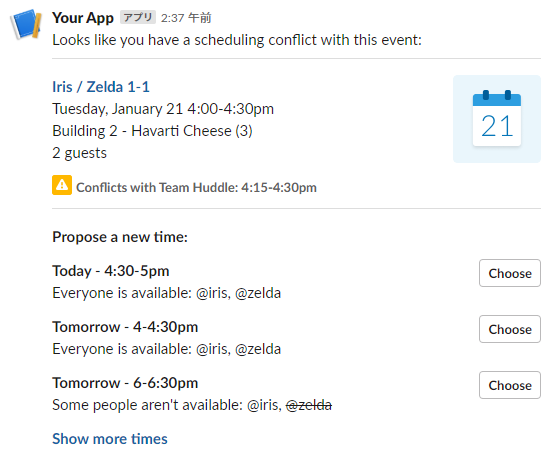
\includegraphics[keepaspectratio, scale=0.7]{images/block_kit_example.png}
 \caption{Block Kitでのメッセージ作成例}
 \label{fig:block_kit_example}
\end{figure}

Block Kitの要素は大きく分けて以下の5つです。

\begin{itemize}
\item Section \\
主にテキストの表示に使用されるが,画像やボタンを含めることもでき,最も自由に扱える要素。
\item Context\\
Sectionとして表示されるよりもサイズが小さく,色が薄いテキスト要素。主に説明などの記載に使用される。
\item Image\\
画像要素。キャプションもつけられる。
\item Divider\\
分割線。
\item Actions\\
ボタンやセレクトボックス,日付セレクタなどのアクション要素。主にSlackとアプリケーション間の双方向通信が可能な場合に使用される。Incoming WebhooksはアプリケーションからSlackへの単方向通信なので,このテキストでは扱わない。
\end{itemize}

Block Kitは,これまでの\verb|text|のみのpayloadではなく,要素ごとにオブジェクトを作成し,それを格納したリストで表現されます。そのため,目的の見た目を実現するためにJSONを手入力で作成するのは骨が折れる作業です。SlackはBlock Kitのプロトタイピングツール\href{https://api.slack.com/tools/block-kit-builder}{Block Kit Builder}を提供しています。これは,GUIを用いてメッセージのひな形を作成できるツールです。


左カラムから追加したい要素を選ぶと,中央カラムにSlackに投稿された際のイメージが表示され,実際のJSONは右カラムに表示されます。右カラムのJSONは編集可能なので,デフォルトの文字列から変更したい場合はこちらを編集して変更します。そのため,Block Kitを利用する場合はBlock Kit Builderを使ってひな形を作り,ひな形をもとにプログラムに落とし込む,といったフローが最も簡単だと思います。

\begin{figure}[H]
 \centering
 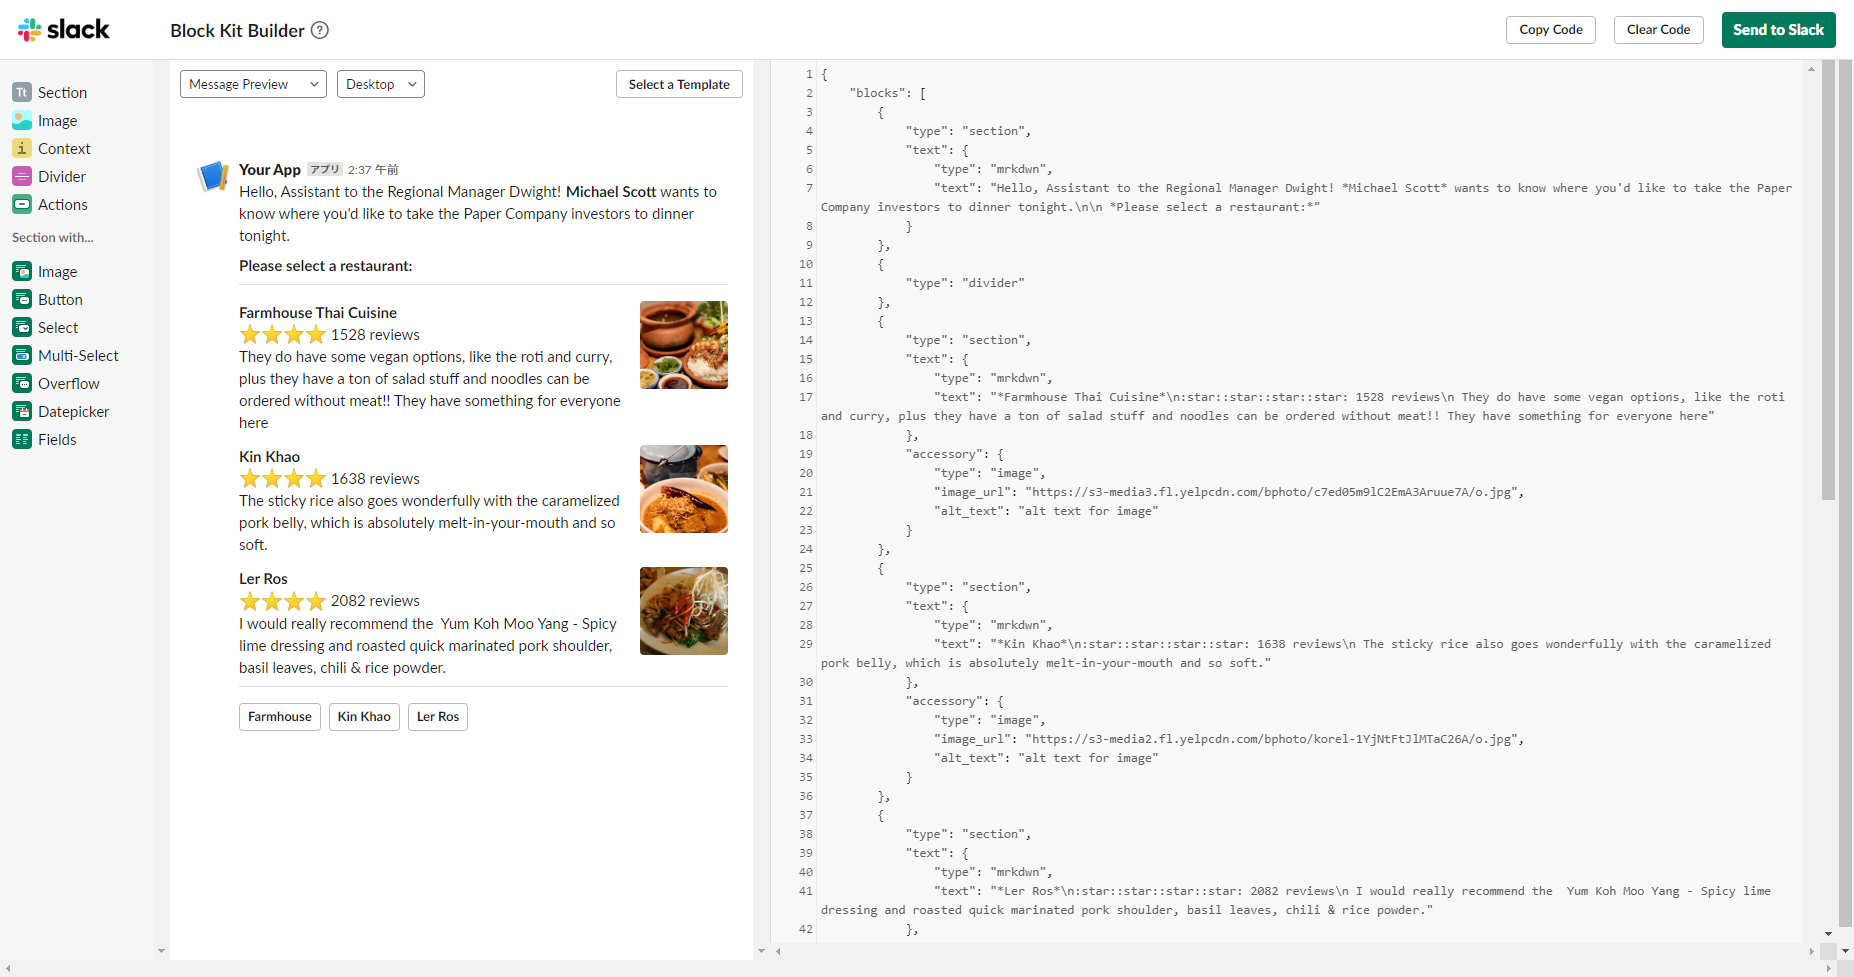
\includegraphics[keepaspectratio, scale=0.35]{images/block_kit_builder.png}
 \caption{Block Kit Builder画面}
 \label{fig:block_kit_builder}
\end{figure}

\subsubsection{Attachments}

Block Kitが登場するまで,このAttachmentsがリッチなメッセージを作成する手段でした。しかし,AttachmentsはBlock Kitの登場によって\textbf{Legacy}とされ,outmoded approach(廃れた手法)とまで記載されるようになってしまいました。

しかし,AttachmentsにできてBlock Kitにはできないことが1つだけあります。それは,``メッセージの左側に色付きのバーを表示すること''です。Attachmentsには,Block Kit BuilderのようなGUIプロトタイピングツールは提供されていませんが,現在のAttachmentsはBlock Kitのラッパーとしても提供されており,Block Kitで作成した\verb|blocks|要素を\verb|attachments|の各要素に入れ込むだけでAttachmentsが利用できます。つまり,AttachmentsはBlock Kitで作成されたメッセージの左側に色付きのバーを追加する機能,として捉えるのがよさそうです。

Attachmentsは,オブジェクトのリストで提供されます。したがって,1つのAttachmentを投稿する場合は,以下のようなpayloadになります。

\begin{lstlisting}[basicstyle=\ttfamily\footnotesize,frame=single,caption=Attachments payload sample]
{
  "text": "Main text",
  "attachments": [
    {
      "color": "#2FA44F",
      "blocks": [
        {
          "type": "section",
          "text": {
            "type": "mrkdwn",
            "text": "This is a block component"
          }
        }
      ]
    }
  ]
}
\end{lstlisting}

\verb|attachments|要素の内容のほとんどがBlock Kitと同様であることがわかります。違いは\verb|color|要素の有無です。このpayloadを使って,Slackにメッセージを投稿すると,以下のように表示されます。

\begin{figure}[H]
 \centering
 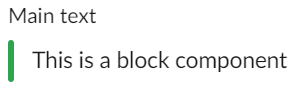
\includegraphics[keepaspectratio, scale=0.8]{images/attachments_sample3.png}
 \caption{Attachmentsを使った投稿例}
 \label{fig:attachments_sample3}
\end{figure}

\section{Google FormsとGAS}

これまではGoogle Apps ScriptとIncoming Webhooksだけを使って,Slackにいろいろなメッセージを投稿してきました。ここからは,実際にGoogle Appsとの連携プログラムを書きます。まずは,Google Formsを題材にGASを作成していきましょう。

この章では,「フォームが送信されたらSlackにその内容を通知する」スクリプトを作成します。Google Formsでは,Google Spreadsheetsに回答内容を蓄積する機能はありますが,Slackへの通知機能はありません。問い合わせフォームや依頼フォームなど,回答が送信されたら即座にキャッチしたいケースは多くあるかと思います。ぜひ,GASを使ってSlack通知を実装してみてください。

\paragraph{本章で扱うトピック}
\begin{itemize}
\item Google Appsに紐づくスクリプトとイベントトリガ
\item Google FormsにおけるEvent Object
\end{itemize}

なお,本テキストではGoogle Formsそのものの利用方法は紹介しません。そのため,断りなしに作成済みのフォームを使用する場合があります。

\subsection{FormApp}

GASにおけるGoogle FormsへのAPIは\verb|FormApp|というクラスで提供されます。\verb|FormApp|は,スクリプトによるフォームの作成,編集,そして参照の手段を提供します。つまり,フォームそのものに対する操作を提供するAPIとなります。実際にフォームから送信された回答を取得する手段は\verb|FormApp|は持っていません。これについては次節\ref{subsec:event_object}以降で扱います。

普段私たちがGoogle Formsでフォームを作成するときはWeb画面からインタラクティブに作成することと思います。わざわざスクリプトを書いてフォームを作成・編集するメリットはイメージしづらいかもしれません。例えば,セレクトボックスの要素を何らかのスプレッドシートやデータベースに記録されている値から動的に生成したい場合などにおいて,スクリプトを用いたフォーム作成が効果を発揮します。ここでも,``Google Formsとスプレッドシート''といった,「異なるサービス間の連携」においてGoogle Apps Scriptが効果を発揮することがわかるかと思います。

\subsubsection{FormAppを使ったフォーム作成}

この項では,テキスト入力形式の質問とセレクトボックス形式の質問を持ったフォームを,Google Apps Scriptで作成してみます。これまでと同様に,Google Apps Scriptのプロジェクトを作成します。今回は,関数名を\verb|createForm|とします。

\begin{lstlisting}[basicstyle=\ttfamily\footnotesize,frame=single,caption=FormApp sample 1]
function createForm() {

}
\end{lstlisting}

画面からフォームを作成する場合も,Google Apps Scriptでフォームを作成する場合も,基本的な流れは変わりません。\textbf{新しいフォームを作成}して,作成したフォームに\textbf{質問を追加}するといった流れです。

まず,新しいフォームを作成する場合は,\verb|FormApp.create()|を使用します。引数には,作成するフォームの名称を入力します。

\begin{lstlisting}[basicstyle=\ttfamily\footnotesize,frame=single,caption=FormApp sample 2]
function createForm() {
  var form = FormApp.create("Sample Form");
}
\end{lstlisting}

上記の状態でスクリプトを実行すると,\verb|Sample Form|という名称で空のフォームが作成されます。なお,このスクリプトは\textbf{実行するごとに新しいフォームが作成されますので,注意が必要です}。

ここから,フォームに対して質問を追加していきます。まずは,テキスト入力形式の質問を追加します。テキスト入力形式の質問には,短文回答(1行)と長文回答(複数行)の2種類があります。今回は,長文回答形式の質問を追加します。

長文回答形式の質問を追加するには,フォームに対して,\verb|addParagraphTextItem()|を実行します。

\begin{lstlisting}[basicstyle=\ttfamily\footnotesize,frame=single,caption=FormApp sample 3]
function createForm() {
  var form = FormApp.create("Sample Form");
  form.addParagraphTextItem()
}
\end{lstlisting}

ここで追加された質問には,タイトルや説明,必須項目か否かなどの情報はまだ設定されていません。\verb|Form.addParagraphTextItem()|の返り値は\verb|ParagraphTextItem|クラスです。このクラスには,以下のようなメソッドがありますので,これを使って設定していきます。

\begin{itemize}
\item \verb|setTitle()|\\
タイトルを設定する
\item \verb|setHelpText()|\\
説明を設定する
\item \verb|setRequired()|\\
必須項目として設定する
\end{itemize}

\begin{lstlisting}[basicstyle=\ttfamily\footnotesize,frame=single,caption=FormApp sample 4]
function createForm() {
  var form = FormApp.create("Sample Form");
  form.addParagraphTextItem()
  .setTitle("Paragraph Text Question")
  .setHelpText("This ParagraphTextItem is automatically created by GAS.")
  .setRequired(true);
}
\end{lstlisting}

上記スクリプトを実行すると,以下の図\ref{fig:form_sample1}のようなフォームが作成されます。

\begin{figure}[H]
 \centering
 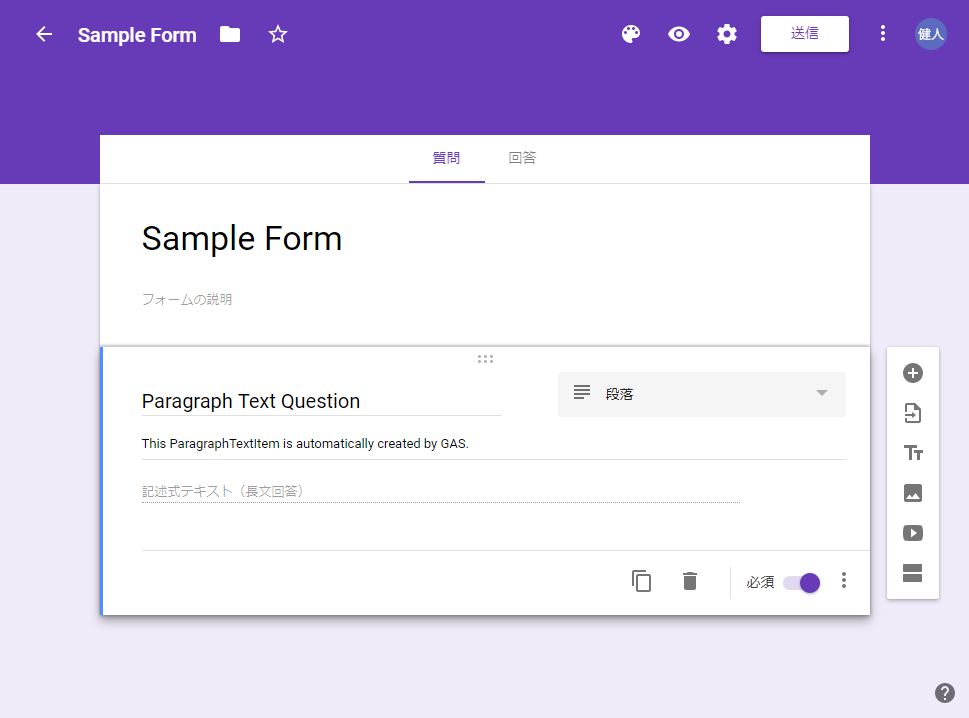
\includegraphics[keepaspectratio, scale=0.5]{images/form_sample1.png}
 \caption{FormAppによるフォームの作成例1}
 \label{fig:form_sample1}
\end{figure}

さらに,セレクトボックス形式の質問を追加していきます。セレクトボックス回答形式の質問を追加するには,フォームに対して,\verb|addListItem()|を実行します。


タイトルや説明の設定は,\verb|ParagraphTextItem|と同様に\verb|setTitle()|,\verb|setHelpText()|で行えます。セレクトボックスにアイテムを追加するのは\verb|ListItem.setChoiceValues()|が最も簡便な手法です。これは,文字列のリストをまとめてアイテムとして追加するメソッドです。

\begin{lstlisting}[basicstyle=\ttfamily\footnotesize,frame=single,caption=FormApp sample 5]
function createForm() {
  var form = FormApp.create("Sample Form");
  
  // 長文回答形式の質問を追加する
  form.addParagraphTextItem()
  .setTitle("Paragraph Text Question")
  .setHelpText("This ParagraphTextItem is automatically created by GAS.")
  .setRequired(true);
  
  // セレクトボックス形式の質問を追加する
  form.addListItem()
  .setTitle("List Question")
  .setHelpText("This ListItem is automatically created by GAS.")
  .setChoiceValues(["hoge", "fuga", "foo", "bar"]);
}
\end{lstlisting}

以上でフォームの作成,質問の追加が完了しました。最終的に作成されたフォームは以下の図\ref{fig:form_sample3}です。
他の質問形式の追加方法など,FormAppのより詳しい情報は,\href{https://developers.google.com/apps-script/reference/forms}{公式ドキュメント}に記載されています。

\begin{figure}[H]
 \centering
 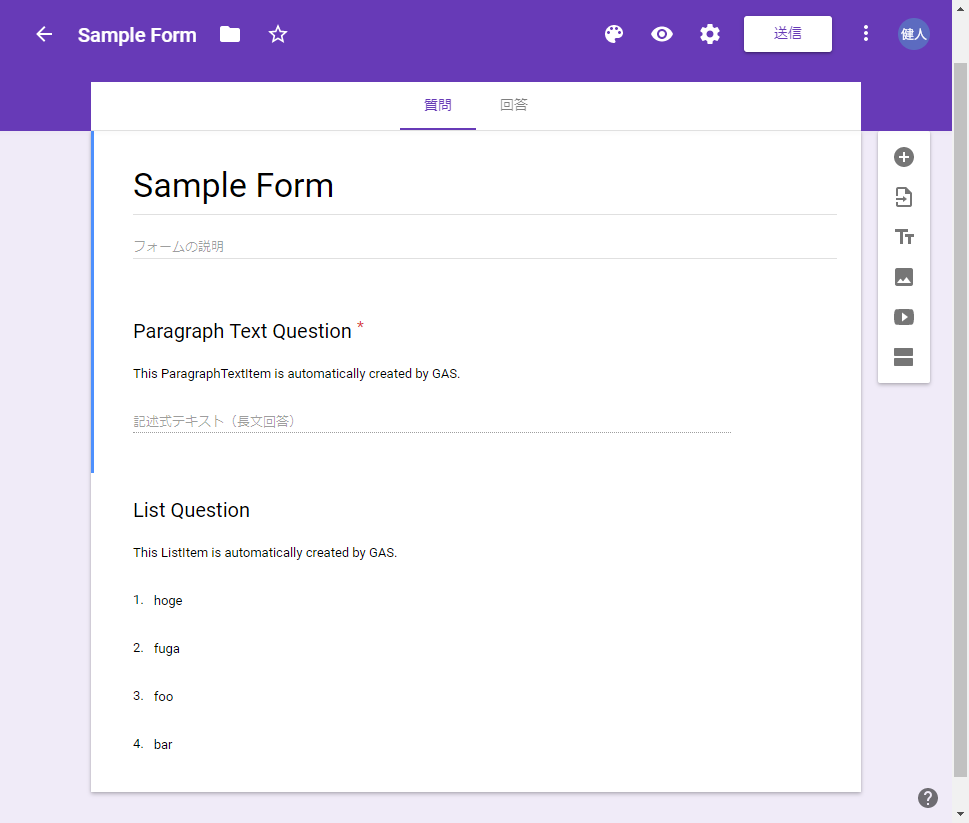
\includegraphics[keepaspectratio, scale=0.5]{images/form_sample3.png}
 \caption{FormAppによるフォームの作成例2}
 \label{fig:form_sample3}
\end{figure}

最後に,作成したフォームのURLを取得する方法を紹介します。作成したフォームのURLは,\verb|form.getPublishedUrl()|と\verb|form.getEditUrl()|から取得できます。それぞれ,実際に公開されるフォームのURLと,フォームの編集画面のURLです。

\begin{lstlisting}[basicstyle=\ttfamily\footnotesize,frame=single,caption=FormApp sample 6]
function createForm() {
  var form = FormApp.create("Sample Form");
  
  // 長文回答形式の質問を追加する
  form.addParagraphTextItem()
  .setTitle("Paragraph Text Question")
  .setHelpText("This ParagraphTextItem is automatically created by GAS.")
  .setRequired(true);
  
  // セレクトボックス形式の質問を追加する
  form.addListItem()
  .setTitle("List Question")
  .setHelpText("This ListItem is automatically created by GAS.")
  .setChoiceValues(["hoge", "fuga", "foo", "bar"]);
  
  Logger.log(form.getPublishedUrl());
  Logger.log(form.getEditUrl());
}
\end{lstlisting}

上記のスクリプトを実行すると,ログに作成されたフォームのURLが表示されます。

\begin{figure}[H]
 \centering
 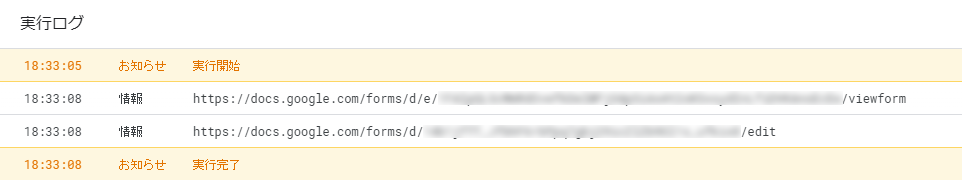
\includegraphics[keepaspectratio, scale=0.5]{images/form_sample2.png}
 \caption{フォームURLの取得例}
 \label{fig:form_sample2}
\end{figure}

\subsection{Google Appsに紐づくスクリプト}
\label{subsec:event_object}

前節では,FormAppを使ってスクリプトからフォームを作成する方法を紹介しました。本節では,既に作成されたフォームから回答が送信されたとき,それを受け取る方法について紹介します。今回は,前節で作成したフォーム(図\ref{fig:form_sample3})を引き続き使用します。

まず,フォーム編集画面右上にある,「\ $\mathbf{\vdots}$\ 」をクリックし,「スクリプト エディタ」を選択します。すると,スクリプト編集画面が開きます。これは,フォームに紐付いたスクリプトになりますので,以降はこちらからスクリプトを編集します。

\begin{figure}[H]
 \centering
 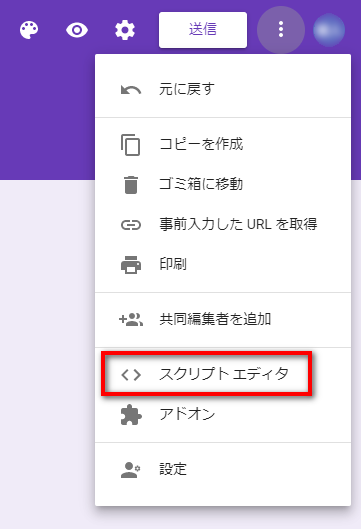
\includegraphics[keepaspectratio, scale=0.5]{images/form_sample4.png}
 \caption{フォームからスクリプトエディタを開く}
 \label{fig:form_sample4}
\end{figure}

\subsubsection{イベントトリガ}
\label{ssub:event_trigger}

フォームをはじめとして,Google Appsに紐づくスクリプトでは,\textbf{イベントトリガ}が使用できます。イベントトリガとは,Google Appsに対するユーザーの\ruby[g]{操作}{イベント}を\ruby[g]{きっかけ}{トリガ}にスクリプトを実行する機能です。フォームであれば,「回答の送信」や「フォームを開く」,スプレッドシートであれば「シートの編集」や「シートの追加」がイベントにあたります。


イベントトリガや,後述する時間主導型トリガなどのトリガ編集画面は,スクリプト編集画面のツールバーから,時計マークのボタンをクリックするとアクセスできます。トリガ編集画面右下に「$+$トリガーを追加」というボタンがあります。これをクリックして,トリガを設定します。

\begin{figure}[H]
 \centering
 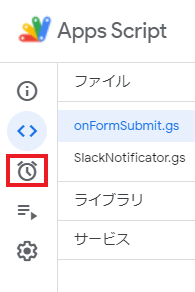
\includegraphics[keepaspectratio, scale=0.7]{images/trigger_button.png}
 \caption{トリガ編集画面を開く}
 \label{fig:trigger_button}
\end{figure}

トリガ設定画面では,以下の項目を設定できます。
\begin{itemize}
\item 実行する関数\\
トリガによって実行される関数を選択します。
\item 実行するデプロイ\\
スクリプトのバージョン管理を行っている場合,ここから実行するバージョンを選択できます。\\
常に最新のスクリプトを実行するのであれば,ここは\verb|Head|のままで大丈夫です。
\item イベントのソース\\
イベントをどこから取得するか選択します。今回は,フォームに回答が送信されたらスクリプトを実行しますので,「フォームから」を選択します。
\begin{itemize}
\item Google Appsから(フォームから)
\item 時間主導型
\item カレンダーから
\end{itemize}
\item イベントの種類\\
「イベントのソース」にて「Google Appsから」を選択した場合,こちらが表示されます。フォームの場合,「起動時」と「フォーム送信時」が選択できます。今回は後者を選択します。
\item エラー通知の頻度\\
トリガによるスクリプトの実行でエラーが発生した場合に,メール通知を行うことができます。以下の頻度から選択できます。
\begin{itemize}
\item 今すぐ通知を受け取る
\item 1時間おきに通知を受け取る
\item 毎日通知を受け取る
\item 1週間おきに通知を受け取る
\end{itemize}
\end{itemize}

今回は,以下のように設定を行いました。

\begin{figure}[H]
 \centering
 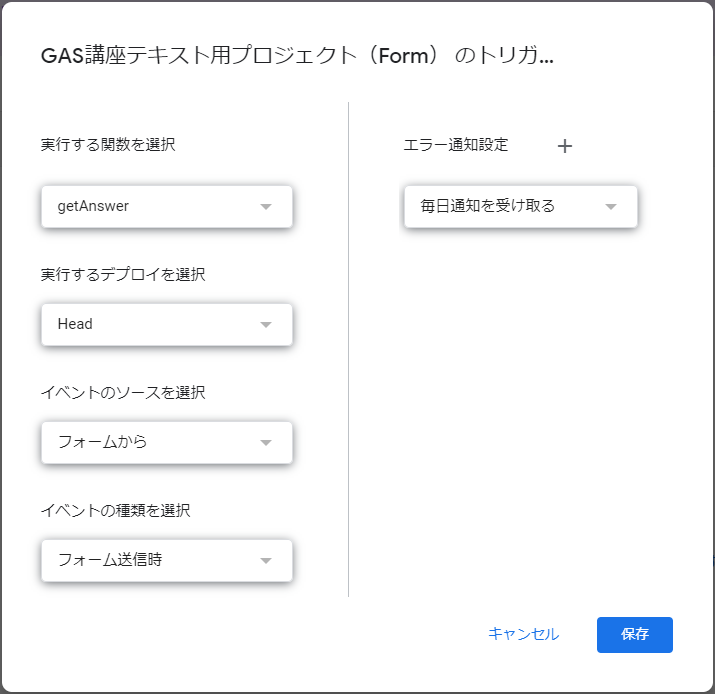
\includegraphics[keepaspectratio, scale=0.7]{images/trigger_edit.png}
 \caption{トリガの設定例}
 \label{fig:trigger_edit}
\end{figure}

\subsubsection{Event Object}

イベントトリガによって実行された関数は,そのイベントに関する情報を関数の引数として受け取ることができます。これを\href{https://developers.google.com/apps-script/guides/triggers/events?hl=en}{Event Object}といいます。Event Objectを受け取るために,実行される関数に引数を設定します。いま,「フォーム送信時」のイベントをトリガとして設定しているので,それに対応する引数として,\verb|formSendEventObject|と名前をつけます。

\begin{lstlisting}[basicstyle=\ttfamily\footnotesize,frame=single,caption=Event Object sample 1]
function getAnswer(formSendEventObject) {
  
}
\end{lstlisting}

Event Objectは,対応するイベントに応じて保持している情報が異なります。フォーム送信イベントによって受け取るEvent Objectにはフォームの回答,スプレッドシートの編集イベントによって受け取るEvent Objectには編集された内容・・・といった具合です。今回はフォーム送信によるEvent Objectを受け取っていますので,\href{https://developers.google.com/apps-script/guides/triggers/events?hl=en#form-submit_1}{こちら}に記載されている通りの内容が含まれています。実際に送信されたフォームの内容は,\verb|response|要素に含まれています。\verb|response|要素には,フォームの回答を格納するための\verb|FormResponse|クラスのオブジェクトが含まれています。\verb|FormResponse|クラスのオブジェクトには,実際に送信された回答の内容,送信された時間,送信した人のメールアドレス\footnote{メールアドレスを収集する設定が有効になっている場合のみ}などが格納されています。まずは,送信された回答を取得してみましょう。

\paragraph{回答の内容を取得する}

実際の回答を取得するには,\verb|FormResponse.getItemResponses()|を実行します。これは,個々の回答を格納するための\verb|ItemResponse|クラスのリストが返ってきます。

\begin{lstlisting}[basicstyle=\ttfamily\footnotesize,frame=single,caption=Event Object sample 2]
function getAnswer(formSendEventObject) {
  var response = formSendEventObject.response;
  var itemResponses = response.getItemResponses();
}
\end{lstlisting}

\verb|itemResponses|変数を\verb|Logger.log(itemResponse)|でログに出力してみましょう。イベントトリガによって実行されるスクリプトのログは,エディタ画面を開いた状態でイベントを起こすと確認できます。


図\ref{fig:form_sample3}のフォームを使用していますので,質問の数は2つです。\verb|itemResponses|をそのままログに出力すると,以下のように出力されます。

\begin{lstlisting}[basicstyle=\ttfamily\footnotesize,frame=single,caption=Event Object output example 1]
[19-12-12 16:34:33:783 JST] [ItemResponse, ItemResponse]
\end{lstlisting}

2つの回答が含まれているので,要素を2つ持ったリストになります。しかし,このままでは\verb|ItemResponse|クラスのオブジェクトが2つあることしか分からず,どのような回答が得られたのかわかりません。


\verb|ItemResponse|オブジェクトから,実際の回答内容を取得するには,\verb|ItemResponse.getResponse()|を実行します。いま,\verb|ItemResponse|オブジェクトのリストとして回答を取得できていますので,以下のようなスクリプトで順にログに出力してみます。

\begin{lstlisting}[basicstyle=\ttfamily\footnotesize,frame=single,caption=Event Object sample 3]
function getAnswer(formSendEventObject) {
  var response = formSendEventObject.response;
  var itemResponses = response.getItemResponses();
  
  for (var i = 0; i < itemResponses.length; i++) {
    Logger.log(itemResponses[i].getResponse());
  }
}
\end{lstlisting}

上記のスクリプトを保存した状態でフォームから回答を送信すると,以下のようなログが出力されます。しかし,今取得できている(ログに表示できている)のは回答の内容のみであり,「どのような質問への回答なのか」が分かりづらく,不親切なログとなってしまっています。


\begin{lstlisting}[basicstyle=\ttfamily\footnotesize,frame=single,caption=Event Object output example 2]
[19-12-12 16:40:10:881 JST] Test Answer
[19-12-12 16:40:10:881 JST] hoge
\end{lstlisting}

そこで,ログに質問のタイトルも出力するようにしてみましょう。\\質問のタイトルは,\verb|ItemResponse.getItem().getTitle()|で取得できます。これは,まず\verb|ItemResponse.getItem()|で質問の内容を持つ\verb|Item|オブジェクトを取得し,それからタイトルを取得しています。ログを読みやすくするため,質問と回答を区別できるような文言を追加し,以下のようなスクリプトを書きます。

\begin{lstlisting}[basicstyle=\ttfamily\footnotesize,frame=single,caption=Event Object sample 4]
function getAnswer(formSendEventObject) {
  var response = formSendEventObject.response;
  var itemResponses = response.getItemResponses();
  
  for (var i = 0; i < itemResponses.length; i++) {
    Logger.log("Question: " + itemResponses[i].getItem().getTitle());
    Logger.log("Answer: " + itemResponses[i].getResponse());
  }
}
\end{lstlisting}

上記スクリプトが実行されると,以下のようなログになります。だいぶ読みやすくなりました。

\begin{lstlisting}[basicstyle=\ttfamily\footnotesize,frame=single,caption=Event Object output example 3]
[19-12-12 00:49:36:146 PST] Question: Paragraph Text Question
[19-12-12 00:49:36:147 PST] Answer: Test Answer
[19-12-12 00:49:36:312 PST] Question: List Question
[19-12-12 00:49:36:314 PST] Answer: hoge
\end{lstlisting}

\paragraph{回答者のメールアドレスを取得する}

次に,回答した人のメールアドレスを取得してみましょう。メールアドレスを取得するには,フォームの設定から「メールアドレスを収集する」にチェックを入れておく必要があります。


回答者のメールアドレスは,\verb|FormResponse.getRespondentEmail()|から取得できます。Works Human Intelligence では,メールアドレスの@前がSlackのUsernameにもなっていますので,回答者にメンションを送るなどといった応用の足がかりになります。

先程のスクリプトに,メールアドレスのログ出力を追加します。

\begin{lstlisting}[basicstyle=\ttfamily\footnotesize,frame=single,caption=Event Object sample 5]
function getAnswer(formSendEventObject) {
  var response = formSendEventObject.response;
  var itemResponses = response.getItemResponses();
  
  Logger.log("RespondentEmail: " + response.getRespondentEmail());
  
  for (var i = 0; i < itemResponses.length; i++) {
    Logger.log("Question: " + itemResponses[i].getItem().getTitle());
    Logger.log("Answer: " + itemResponses[i].getResponse());
  }
}
\end{lstlisting}

上記スクリプトを実行すると,以下のようなログが出力されます。メールアドレスが正しく取得できることが確認できます。

\begin{lstlisting}[basicstyle=\ttfamily\footnotesize,frame=single,caption=Event Object output example 4]
[19-12-12 17:56:50:299 JST] RespondentEmail: shimada_ken@example.com
[19-12-12 17:56:50:441 JST] Question: Paragraph Text Question
[19-12-12 17:56:50:442 JST] Answer: Test Message
[19-12-12 17:56:50:535 JST] Question: List Question
[19-12-12 17:56:50:536 JST] Answer: hoge
\end{lstlisting}


\verb|FormResponse|クラスには,他にもいろいろな情報が格納されています。詳細は\href{https://developers.google.com/apps-script/reference/forms/form-response?hl=en}{こちら}から確認できます。

\subsection{質問形式と取り出され方}


前節では,文字列形式の回答と択一方式の回答についてログに出力してみました。フォームには他にも複数選択可能な質問(チェックボックスなど)や,日時を選択する質問など,様々な形式の質問があります。これらの回答をスクリプトで取り出すとどうなるか確認してみましょう。

図\ref{fig:various_question}のような,様々な形式の質問をもったフォームを作成してみました。これの回答を先ほどと同様にログに出力してみます。

\begin{figure}[H]
 \centering
 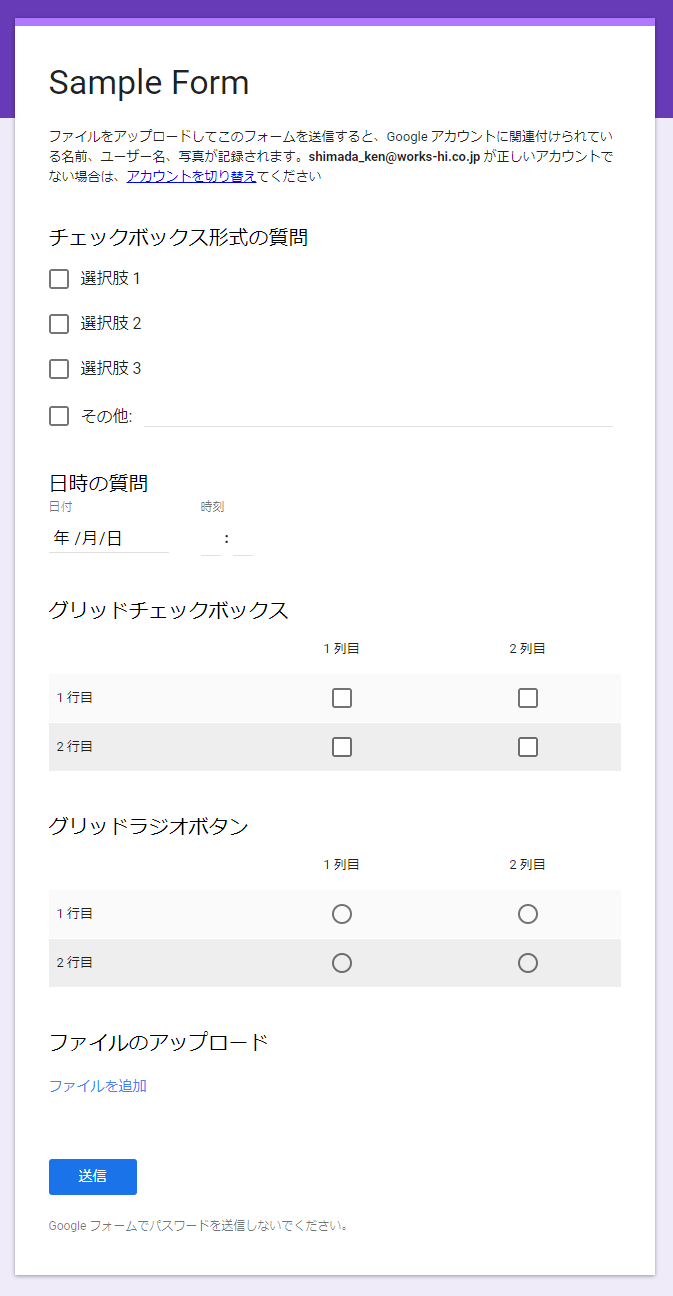
\includegraphics[keepaspectratio, scale=0.5]{images/various_question.png}
 \caption{いろいろな形式の質問を持ったフォーム}
 \label{fig:various_question}
\end{figure}

上記のようなフォームの回答をスクリプトから取り出すと,以下のような結果が取得できます。

\begin{lstlisting}[basicstyle=\ttfamily\footnotesize,frame=single,caption=Event Object sample 6]
[19-12-12 01:40:55:372 PST] RespondentEmail: shimada_ken@example.com
[19-12-12 01:40:55:446 PST] Question: チェックボックス形式の質問
[19-12-12 01:40:55:447 PST] Answer: 選択肢 2,その他
[19-12-12 01:40:55:520 PST] Question: 日時の質問
[19-12-12 01:40:55:521 PST] Answer: 2019-12-12 12:34
[19-12-12 01:40:55:610 PST] Question: グリッドチェックボックス
[19-12-12 01:40:55:610 PST] Answer: 1 列目,2 列目,2 列目
[19-12-12 01:40:55:676 PST] Question: グリッドラジオボタン
[19-12-12 01:40:55:677 PST] Answer: 1 列目,2 列目
[19-12-12 01:40:55:744 PST] Question: ファイルのアップロード
[19-12-12 01:40:55:745 PST] Answer: 1P0g8_AFoWIob4uFeHxQ9ZnUK3eo_Jqyw
\end{lstlisting}


質問の回答は,\verb|String|,\verb|String[]|,または\verb|String[][]|のいずれかの形式で取得されます。基本的には\verb|String|で取得されますが,複数の回答を持ちうる以下の3つは\verb|String[]|または\verb|String[][]|で取得されます。詳細は\href{https://developers.google.com/apps-script/reference/forms/item-response.html?hl=en#getResponse()}{こちら}。
\begin{itemize}
\item \verb|CheckboxItem|(チェックボックス形式の質問)\\
この回答は\verb|String[]|(文字列のリスト)で返ってきます。
\item \verb|GridItem|(グリッドラジオボタン)\\
この回答も\verb|String[]|で返ってきます。\verb|[1行目の回答, 2行目の回答, ...]|といった具合です。
\item \verb|CheckboxGridItem|(グリッドチェックボックス)\\
この回答は,各行で複数の回答が選択されうるので,唯一\verb|String[][]|(文字列の2次元リスト)で返ってきます。\\
$i$行目の$j$番目の回答を$A_{i, j}$とすると,$\left[\left[A_{1, 1}, A_{1, 2}, \dots\right], \left[A_{2, 1}, A_{2,2}, \dots\right], \dots\right]$といった形です。
\end{itemize}

また,「ファイルのアップロード」の質問の取り出され方には少し注意が必要です。上記ログの最終行を見るとわかるように,謎の文字列が返ってきているように見えます。これは\textbf{ファイルID}と呼ばれる値で,Google Driveにアップロードされるファイルに一意に与えられる文字列です。Google Driveで,なんらかのファイルの共有リンクを取得してみてください。\verb|https://drive.google.com/open?id={ファイルID}|というURLが取得できると思います。この``\verb|id=|''以下の文字列がファイルIDです。Google DriveにアップロードされたファイルのURLはファイルIDで識別されていますので,逆にファイルIDさえあれば,実際にブラウザからファイルにアクセスするためのURLを特定できます。

ちなみに,ファイルIDのみならず,スプレッドシートやスライド,フォームなど,Google Appsで作成したものにはすべてIDが割り当てられています。

\clearpage

\subsection{Practice: Google Forms $\times$ Slack}

本章では,Google FormsをGASから扱う方法について説明してきました。また,前章ではGASからSlackへメッセージを投稿する方法について説明しました。これらを組み合わせて,\textbf{図\ref{fig:practice_form}に示すようなフォームを作成し,回答が送信されたら,その内容をSlackに送信する}スクリプトを作成してみましょう。

作成例は本テキストの付録に記載しています。これが唯一の正解というわけではないので,参考程度にとどめておいてください。

\begin{figure}[H]
 \centering
 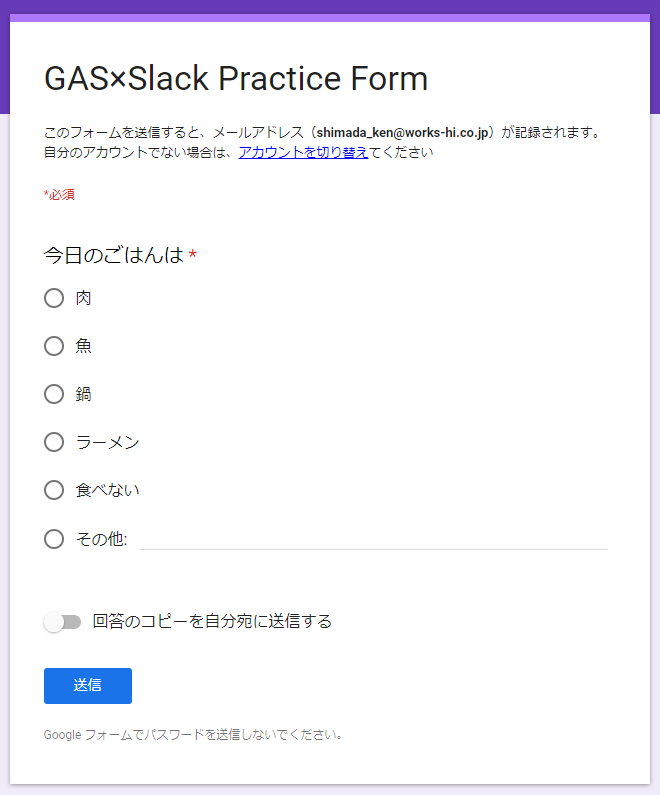
\includegraphics[keepaspectratio, scale=0.5]{images/practice_form.png}
 \caption{対象となるフォーム}
 \label{fig:practice_form}
\end{figure}

\clearpage

\section{Google SpreadsheetsとGAS}

本章では,Google Spreadsheetsを操作するGASについて紹介します。

\paragraph{本章で扱うトピック}
\begin{itemize}
\item Spreadsheetの構造
\item SpreadsheetApp
\item 時間主導型トリガ
\end{itemize}

\subsection{Spreadsheet の構造 - プログラムでスプレッドシートを扱うとはどういうことか}


普段私たちがスプレッドシートを扱うとき,その構造について意識することはありません。といっても,実際にはスプレッドシートというアプリケーションそのものはその構造の上に成り立っています。なぜ私たちがこの構造を意識せず使用できるかというと,構造を視覚を用いて無意識的に認識しているからにほかなりません。

しかし,プログラムは視覚を持ちません。ですので,これからプログラムを作成する私たちはスプレッドシートの構造について改めて認識する必要があります。

さて,スプレッドシートは何から構成されているでしょうか?大まかに分けると,以下のような要素から構成されています。

\begin{itemize}
\item スプレッドシート全体
\item シート
\item 行や列
\item セル
\item 値
\end{itemize}

これらは,上から下に向かって包含関係を持ちます。つまり,「スプレッドシート全体」には1つ以上の「シート」が含まれ,「シート」には1つ以上の「行や列」が含まれ・・・といった関係です。スプレッドシート上のある「値」をプログラムを使って取り出す場合は,この包含関係を意識する必要があります。

つまり,いきなり「値」を取り出すことはできないので,「スプレッドシート全体」を取ってきて,そこから「シート」を取ってきて,そこから「行や列,セル」を取ってきて,ようやく「セル」の中にある「値」にアクセスできます。マトリョーシカのように順番に取り出すしかないのです。マトリョーシカのように\footnote{大事なことなので2回言いました}。


\begin{figure}[H]
 \centering
 
\includegraphics[keepaspectratio, scale=0.5]{images/spreadsheet_matryoshka.pdf}
 \caption{プログラムでスプレッドシートから値を取り出す順序(イメージ)}
 \label{fig:spreadsheet_matryoshka}
\end{figure}


% However, I told ``we recognize the spreadsheet structure unconsciously''. Concrete example is; When if you want to access a value in some spreadsheet, you may search the target spreadsheet from your bookmark, Google Drive, link url, etc... at first. After that, when you open the spreadsheet, you'll select the target sheet from its name. Then you see the sheet, you'll search the value by using your own eyes. It is absolutely same as the way of program!

ところで,先程``私たちは(スプレッドシートの)構造を視覚を用いて無意識的に認識している''と説明しました。この具体的な例について紹介しましょう。


あなたがあるスプレッドシートに記録されている情報を確認したいとき,以下のような行動を取ると思います。
\begin{enumerate}
\item まず,対象のスプレッドシートを開こうと,ブックマークやGoogle Spreadsheetsのトップページを参照します。
\item 対象のスプレッドシートを開いたら,(シートが複数ある場合)シート名から対象のシートを選択します。
\item 対象のシートを開いたら,視覚を用いて目的の情報を探します。
\end{enumerate}

上記のフローはプログラムが行っている方法とほぼ同じと言えます。しかし,この構造について意識することは普段ありません。


\subsection{SpreadsheetApp}


フォームを操作するクラスが\verb|FormApp|だったように,スプレッドシートを操作するクラスは\verb|SpreadsheetApp|です。「Excel方眼紙」「ネ申Excel」などと揶揄されるように\footnote{ググるといろいろな議論が出てくる。},スプレッドシートは単なる表計算に収まらない非常に自由な表現が可能です。したがって,\verb|SpreadsheetApp|ができる操作も非常に多く,その全てをこのテキストで紹介することはできません。本テキストでは,Slackとの連携に主軸を置いているため,特にスプレッドシートから値を取り出す方法を中心に\verb|SpreadsheetApp|の扱い方について説明します。

本節では,出席管理や,集金管理などを行うシートを想定して,以下の図\ref{fig:spreadsheet_sample}に示すようなスプレッドシートの値をスクリプトから取得する方法について説明します。

\begin{figure}[H]
 \centering
 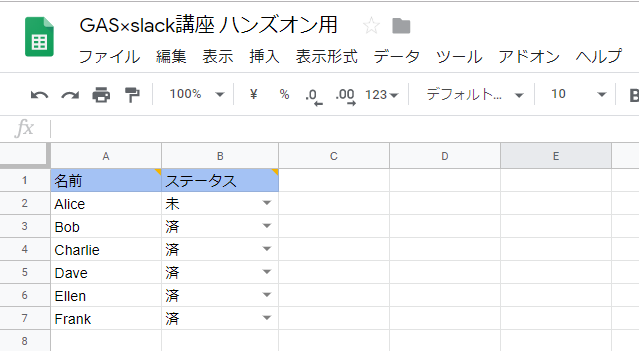
\includegraphics[keepaspectratio, scale=0.7]{images/spreadsheet_sample.png}
 \caption{スプレッドシート例}
 \label{fig:spreadsheet_sample}
\end{figure}

前節にて説明したように,スクリプトからスプレッドシートを扱う際には構造に併せて順番に参照する必要があります。したがって,スプレッドシートからある値を取り出すには,以下のような流れで処理を記述します。

\begin{enumerate}
\item スプレッドシートを取得する
\item スプレッドシートからシートを取得する
\item シートから範囲(または1つのセル)を取得する
\item 範囲(または1つのセル)から値を取得する
\end{enumerate}

まず,スプレッドシートを取得してみましょう。

\subsubsection{スプレッドシートを取得する}

% SpreadsheetApp.openById, SpreadsheetApp.openByUrl, ss.getSheets, ss.getSheetByName, sheet.getRange, sheet.getSheetValues. 

スプレッドシートは,Google DriveのファイルIDと同様に,\verb|スプレッドシートID|で一意に識別されます。したがって,スプレッドシートIDから特定のスプレッドシートを指定し,スクリプトから呼び出すことが可能です。スプレッドシートIDからスプレッドシートを取得するには,\verb|SpreadsheetApp.openById()|を使います。

スプレッドシートIDは,スプレッドシートのURLから確認できます。スプレッドシートのURLは\verb|https://docs.google.com/spreadsheets/d/{スプレッドシートID}/edit|のようになっており,\verb|{スプレッドシートID}|の部分にスプレッドシートIDがあります。

GASのスクリプトエディタを開き,まずはスプレッドシートを取得する処理を書きます。

\begin{lstlisting}[basicstyle=\ttfamily\footnotesize,frame=single,caption=SpreadsheetApp sample 1]
function spreadsheetSample() {
  var spreadsheet = SpreadsheetApp.openById('Spreadsheet ID');
}
\end{lstlisting}

また,URLからスプレッドシートIDを抽出せずとも,URLを直接指定してスプレッドシートを取得することも可能です。その場合は,\verb|SpreadsheetApp.openByUrl()|を使用します。

\begin{lstlisting}[basicstyle=\ttfamily\footnotesize,frame=single,caption=SpreadsheetApp sample 2]
function spreadsheetSample() {
  var spreadsheet = SpreadsheetApp.openByUrl('https://docs.google.com/spreadsheets/d/{Spreadsheet ID}/edit');
}
\end{lstlisting}

\subsubsection{スプレッドシートからシートを取得する}


前項で取得したスプレッドシートから,特定のシートを取得してみましょう。シートには名前がついています。これは,スプレッドシートにおいて一意\footnote{同じスプレッドシートに同じ名前のシートを複数作成することはできない}なので,これを使ってシートを特定し,取得できます。シート名を使ってスプレッドシートからシートを取得するには,\verb|Spreadsheet.getSheetByName()|を使います。
いま,図\ref{fig:spreadsheet_sample}のシートには``管理票''という名前がついていますので,以下のようなスクリプトで取得します。

\begin{lstlisting}[basicstyle=\ttfamily\footnotesize,frame=single,caption=SpreadsheetApp sample 3]
function spreadsheetSample() {
  var spreadsheet = SpreadsheetApp.openByUrl('Spreadsheet ID');
  var sheet = spreadsheet.getSheetByName('管理票');
}
\end{lstlisting}

対象としているスプレッドシートに複数のシートがあって,それらをまとめて取得したい場合は\verb|Spreadsheet.getSheets()|が有効です。これは,スプレッドシートにあるシート全てを含むリストを取得することができます。

\subsubsection{シートから指定した範囲のセル/値を取得する}


前項で取得したシートから,指定した範囲のセル,もしくは値を取得しましょう。

\begin{itembox}[l]{セルと値の違い}

あるセルに\verb|100|と書かれていた場合を考えてみます。このセルは\verb|100|という値以外にも,様々な情報を持っています。例えば背景色や文字色,フォントタイプ,サイズ,罫線の有無・・・といった具合です。


「セル」はこれらの情報を包含する概念ですが,「値」はその「セル」がもつ\verb|100|という値そのものを指します。

\end{itembox}

指定した範囲のセルを取得する場合は,\verb|Sheet.getRange()|を使います。しかし,今回興味の対象はそのセルに格納されている値ですので,より簡便な\verb|Sheet.getSheetValues()|を使います。

これら2つのメソッドは\verb|row, column, numRows, numColumns|という共通する4つの引数を取ります\footnote{厳密には\verb|getSheetValues|の引数名は\verb|startRow, startColumn, numRows, numColumns|だが,役割はだいたい同じ。}。これらは以下の意味を持ちます。

\begin{itemize}
\item \verb|row|\\
取得する範囲(四角形)の左上の行番号
\item \verb|column|\\
取得する範囲(四角形)の左上の列番号\\
A列が1, B列が2,...と,整数値で指定する。
\item \verb|numRows|\\
\verb|row|行\verb|column|列から何行取得するか
\item \verb|numColumns|\\
\verb|row|行\verb|column|列から何列取得するか
\end{itemize}

言葉で説明すると上記のようになるのですが,いまいち分かりづらいかと思います。そこで,以下の図\ref{fig:getsheetvalues_image}をベースにもう少し詳しく説明してみます。


いま,図に示したようなスプレッドシートがあり,セルB2を左上として5行4列の範囲を取得したいとします。左上のセルB2は上記の引数\verb|row, column|の形式に合わせるとそれぞれ2, 2となります。一方,取得する行数と列数はそれぞれ5, 4ですので,実際に\verb|Sheet.getSheetValues(row, column, numRows, numColumns)|に与えるべき値は2, 2, 5, 4となります。

\begin{figure}[H]
 \centering
 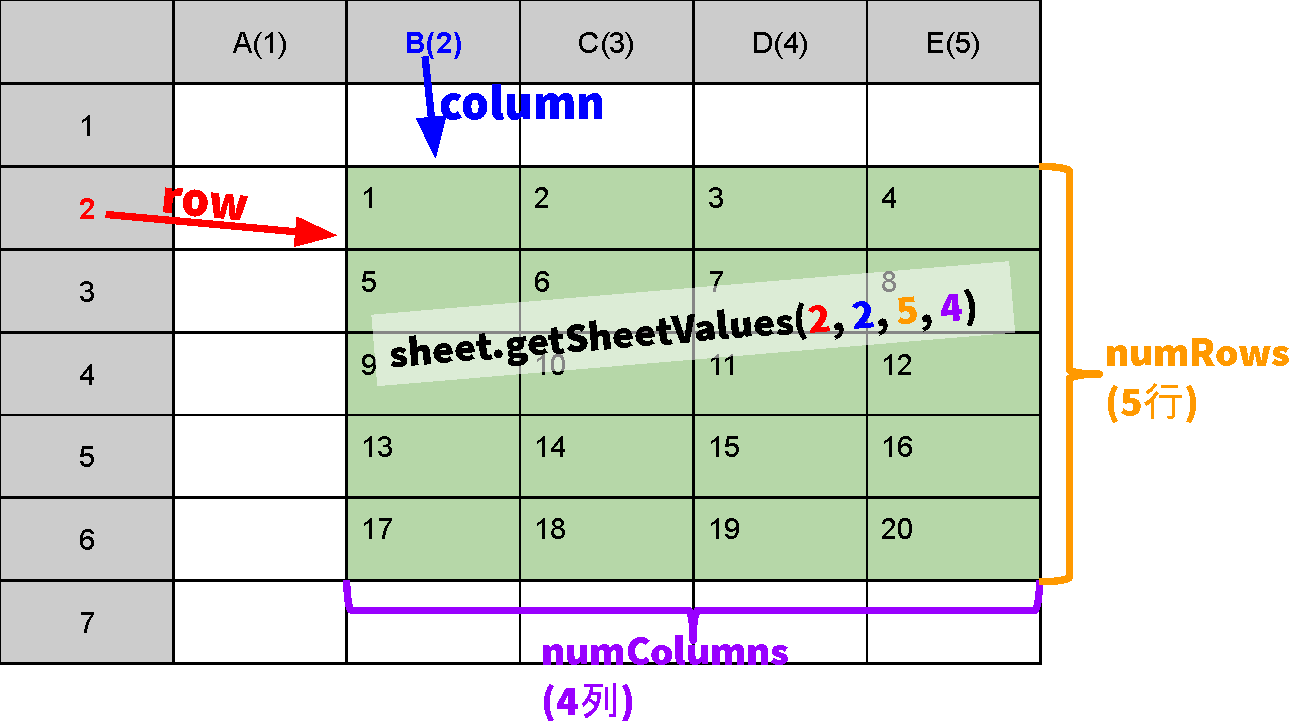
\includegraphics[keepaspectratio, scale=0.7]{images/getsheetvalues_image.pdf}
 \caption{getSheetValuesのイメージ図}
 \label{fig:getsheetvalues_image}
\end{figure}

さて,改めて図\ref{fig:spreadsheet_sample}のスプレッドシートに戻り,取得する範囲と実際に与える引数の値について考えてみましょう。1行目はヘッダ行ですので,スクリプトが取得する必要はありません。したがって,\textbf{2行目1列目}から,\textbf{6行},\textbf{2列}取得すれば良さそうです。よって,与えるべき値は\verb|Sheet.getSheetValues(2, 1, 6, 2)|となります。

\begin{lstlisting}[basicstyle=\ttfamily\footnotesize,frame=single,caption=SpreadsheetApp sample 4]
function spreadsheetSample() {
  var spreadsheet = SpreadsheetApp.openByUrl('Spreadsheet ID');
  var sheet = spreadsheet.getSheetByName('管理票');
  var values = sheet.getSheetValues(2, 1, 6, 2);
  
  Logger.log(values);
}
\end{lstlisting}

実際,上記のスクリプトを実行すると,以下のようなログが確認でき,正しく値が取得できていることが確認できます。ここで注意しておきたいのは,実際に\verb|Sheet.getSheetValues|に引数を与える際には行・列の番号が1から始まるのに対して,実際に取得されるリストのインデックスは0から始まる点です。1-originと0-originを行き来することになりますので,少し注意が必要です。

\begin{lstlisting}[basicstyle=\ttfamily\footnotesize,frame=single,caption=SpreadsheetApp output sample 1]
[19-12-13 19:29:53:321 JST] [[Alice, 未], [Bob, 済], [Charlie, 済], [Dave, 済], [Ellen, 済], [Frank, 済]]
\end{lstlisting}

\begin{itembox}[l]{0-originと1-origin}

ある集合があったとき,その要素を0から数えるのか,それとも1から数えるのか,これを一般に\textbf{オリジン}と呼びます\footnote{日本語圏で多く使われる表現であり,英語圏ではzero-based, one-basedと言うことが多い}。

例えば,年月日はそれぞれ「元年」「1月」「1日」から数えますので,これは1-originとなります。一方で,時間は「0時」「0分」「0秒」から数えますので,これは0-originとなります。

プログラミングにおいては配列・リストの添字(インデックス)は0-originであることが多いです。また,JavaScriptの\verb|Date|クラスでは,月は0-origin,日は1-originと,異なるオリジンが混在します。複数のオリジンを行き来するケースはしばしばありますので,慣れておくとよいです。

\end{itembox}


さて,先程\verb|Sheet.getSheetValues|に引数を与えて,今値が入力されている「6行分」の値を取得することができました。しかし,そもそも「6行」取得したかったのではなく,\textbf{始点の行から末尾の行まで}取得したいはずです。例えば,この管理票で管理する対象の人が増えたとき,スクリプトで\verb|getSheetValues|に与えている値をいちいち書き換えることになってしまいます。これではわざわざスクリプトを書いた意味がなくなってしまいます。

そこで,取得する行数を常に自動的に取得してくれるようにします。末尾の\footnote{値が入っているセルがある最後の行を意味する}行を取得するには,\verb|Sheet.getLastRow()|を使います。図\ref{fig:spreadsheet_sample}の例で言うと,7行目が末尾になりますので,このメソッドを実行すると7が返ってきます。

2行目から範囲を指定していますので,実際に\verb|Sheet.getSheetValues|に渡す際にはヘッダ行分の1を減ずる必要があります。したがって,\verb|Sheet.getSheetValues(2, 1, sheet.getLastRow() - 1, 2)|となります。

したがって,最終形としては以下のようになります。このスクリプトを実行すると,先程と同様なログが出力されます。行をいくつか追加しても,正しく末尾まで取得できることを確認してみましょう。

\begin{lstlisting}[basicstyle=\ttfamily\footnotesize,frame=single,caption=SpreadsheetApp sample 5]
function spreadsheetSample() {
  var spreadsheet = SpreadsheetApp.openByUrl('Spreadsheet ID');
  var sheet = spreadsheet.getSheetByName('管理票');
  var values = sheet.getSheetValues(2, 1, sheet.getLastRow() - 1, 2);
  
  Logger.log(values);
}
\end{lstlisting}

\subsection{Practice: Google Spreadsheets $\times$ Slack}

本章では,スプレッドシートから指定した範囲の値を取得することを中心に,\verb|SpreadsheetApp|の利用方法について説明してきました。ここに,Slackへのメッセージ投稿の処理を組み合わせて,簡易的なリマインダを作成してみましょう。

さきほどの管理票の名前の部分をSlackのユーザ名にかえて,ステータスが\textbf{未}の人に定期的にメンションを送るbotを作ってみてください。

ちなみに,簡単なリマインダであれば,slackの\verb|/remind|コマンドで実現できることもあります。もしGoogle SpreadsheetsとGoogle Apps Scriptでslackリマインダを作る場合は,\verb|/remind|で実現可能か検討してから取り掛かったほうがよいでしょう。

\subsubsection{時間主導型トリガ}

定期的にスクリプトを実行させるには,\textbf{時間主導型トリガ}を使います。前章(\ref{ssub:event_trigger})で説明したとおり,トリガはスクリプトエディタの時計マークのボタンをクリックすると設定できます。

Google Formsのスクリプトの際はイベントトリガを設定しましたが,今回は時間主導型のトリガを設定します。


図\ref{fig:time_based_trigger}に示すように,「イベントのソース」を「時間主導型」とし,トリガーを設定します。「時間ベースのトリガーのタイプ」には実行間隔を設定します。実行間隔には,以下の6種類があります。

\begin{itemize}
\item 特定の日時\\
特定の日時に1度だけ実行します。スクリプトの実行予約のようなイメージです。
\item 分ベースのタイマー\\
数分おきに実行します。間隔は以下の5つから選択できます。
\begin{itemize}
\item 1分おき
\item 5分おき
\item 10分おき
\item 15分おき
\item 30分おき
\end{itemize}
\item 時間ベースのタイマー\\
数時間おきに実行します。間隔は以下の6つから選択できます。
\begin{itemize}
\item 1時間おき
\item 2時間おき
\item 4時間おき
\item 6時間おき
\item 12時間おき
\end{itemize}
\item 日付ベースのタイマー\\
毎日,指定した時間帯に実行します。時間帯は,午前/午後n時台というように設定できます。
\item 週ベースのタイマー\\
毎週何曜日の何時台に実行する,といった形で実行できます。
\item 月ベースのタイマー\\
毎月何日の何時台に実行する,といった形で実行できます。
\end{itemize}

上に示したリストからわかるように,「特定の時間」に実行する方法は「特定の日時」トリガーしかなく,「特定の時間に定期的に実行する」といったトリガーの設定方法は存在しません\footnote{ちなみに,頑張れば実現できます。see: https://qiita.com/chihiro/items/d23692c308c89e1b1ee2}。これは,実際にスクリプトが実行されるサーバー側の負荷分散のための制約です。

\begin{figure}[H]
 \centering
 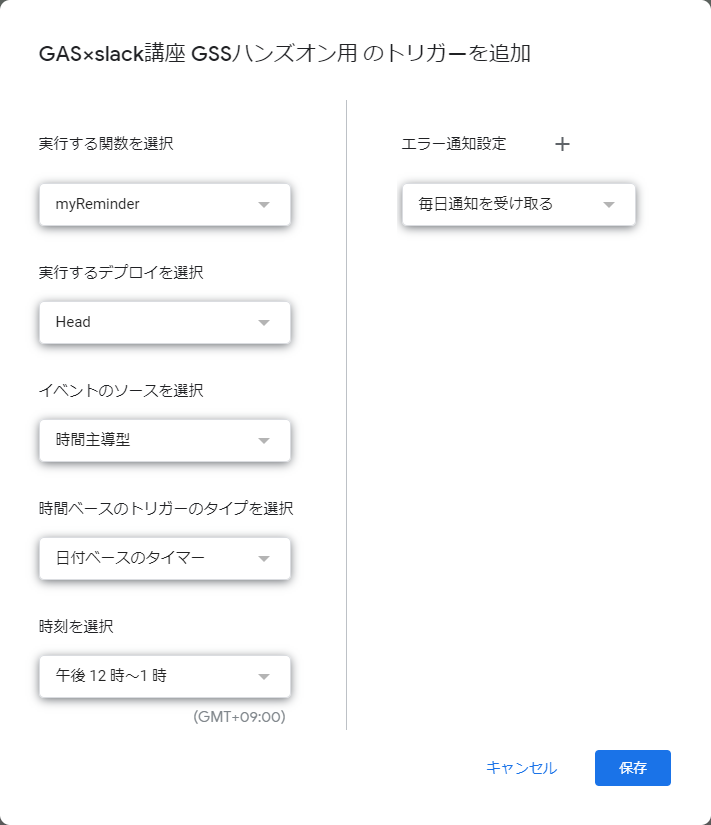
\includegraphics[keepaspectratio, scale=0.7]{images/time_based_trigger.png}
 \caption{時間主導型トリガ}
 \label{fig:time_based_trigger}
\end{figure}

\section{Advanced Practice: Google Forms $\times$ Google Spreadsheets $\times$ Slack}

% ``既存のスプレッドシート''に対して,フォームの回答を転記し,Slackへの通知も行うGASの作成。(CU意見・要望フォームのケース)

ここまで,Google Forms,Google Spreadsheetsを題材に,Google Apps Scriptの扱いかたについて説明してきました。また,練習問題を通して,あるGoogle AppsをGoogle Apps Scriptから操作する方法について学習しました。

発展的な課題として,Google Apps Scriptから,Google FormsとGoogle Spreadsheetsのふたつを同時に操作するスクリプトを書いてみましょう。

\paragraph{作成例} 
何らかの``既存のスプレッドシート''があったとします。そこに,フォームからの回答を転記し,Slackへの通知も行うスクリプトを書いてみましょう。想定されるケースとしては,「今までスプレッドシートに直接記入してもらっていたものをフォームに置き換えた」というケースです。

\section{おわりに}


ちょっとしたプリント程度の分量で収まると思ったら,全然収まりませんでした。修士論文以来,都合2年ぶりに\LaTeX でドキュメントを書いてみました。やっぱり\LaTeX はきれいなドキュメントが簡単に作成できるのでよいですね。


さて,今回取り扱った内容は,Google Apps Script,Incoming Webhooks共にイロハのイ程度の内容です。これらでできることはまだまだ沢山あります。一方で,どちらも公式ドキュメントが英語でしか提供されていないことが学習の障壁になっていますが,テクニカル系のドキュメントは比較的平易な英語で書かれているので,食わず(読まず)嫌いせずに読んでみましょう。ちなみに,世の中には「公式ドキュメント読めば5分で解決することで5時間もGoogleとにらめっこするな」という言葉があります\footnotemark。
\footnotetext{この言葉の出典となったnoteの記事はリンク切れしてしまったので,類似のこちらを紹介します。『私たちはどうして公式ドキュメントが読めないのか?』( https://qiita.com/hiraike32/items/f0a211cceb0ecc516b6c )}

\clearpage
\appendix

\section{実装例}

\subsection{Practice: Google Forms $\times$ Slack}

例えば,以下のような実装例がある。少し投稿されるメッセージの内容を作り込んでいるが,だいたいこんな感じ。なんでもかんでも\verb|var|で宣言するんじゃないとか言わない。ていうかそもそもGoogle Apps Scriptには\verb|let|がない\footnote{ランタイムをV8にすれば\verb|let|が使えます。}。

\begin{lstlisting}[basicstyle=\ttfamily\footnotesize,frame=single,caption=Script Example for Forms practice]
function gasFormPractice(eventObj) {
  var response = eventObj.response;
  var answers = response.getItemResponses();
  
  var answer = answers[0].getResponse();
  
  var email = response.getRespondentEmail();
  var mention = '<@' + email.replace('@example.com','') + '>';
  
  const WEBHOOK = '{Webhook URL}';
  
  var text = ':secret:' + mention + ' さんの今日のお昼は【' + answer + '】らしい';
  
  var params = {
    'method': 'POST',
    'headers': {'Content-type':'application/json'},
    'payload': JSON.stringify({'text': text})
  }
  
  UrlFetchApp.fetch(WEBHOOK, params)
}
\end{lstlisting}

\subsection{Practice: Google Spreadsheets $\times$ Slack}


\begin{lstlisting}[basicstyle=\ttfamily\footnotesize,frame=single,caption=Script Example for Spreadsheets practice]
function myReminderForText() {
  
  const ss = SpreadsheetApp.openById("Spreadsheet ID");
  const sheet = ss.getSheetByName("管理票");
  
  const sheetValues = sheet.getSheetValues(2, 1, sheet.getLastRow()-1, 2);
  
  var attachments = []
  
  for (var value in sheetValues) {
    if (sheetValues[value][1] == '未') {
      attachments.push({'title': 'ステータス未入力ですよ!', 'text': '<@'+sheetValues[value][0]+'>', 'color': '#D50200'})
    }
  }
  
  const WEBHOOK = "{Webhook URL}";
  
  var params = {
    'method': 'POST',
    'headers': {'Content-type':'application/json'},
    'payload': JSON.stringify({'text': '','attachments':attachments})
  }
  
  UrlFetchApp.fetch(WEBHOOK, params)

}
\end{lstlisting}

\begin{figure}[H]
 \centering
 
\includegraphics[keepaspectratio, scale=0.7]{images/spreadsheet_practice_exec_example.png}
 \caption{実行結果}
 \label{fig:spreadsheet_practice_exec_example}
\end{figure}

\section{更新履歴}

v1.0(2019/12/18): 初版公開。

\end{document}